\documentclass[../../main/thesis_msc.tex]{subfiles}


\begin{document}

\chapter{Helium Stars as Progenitors of Thermonuclear Supernovae}

\begin{center}
\textbf{Savvas Chanlaridis}, John Antoniadis, G\"otz Gr\"afener, and Norbert Langer (2019, in prep)
\newline
\end{center}


\begin{center}
\textbf{\large Abstract}
\end{center}
		
Type Ia supernovae (SNe\,Ia) are luminous optical transients characterized by the absence of hydrogen and helium in their spectra. 
The majority of SNe\,Ia are thought to result from the thermonuclear disruption of white dwarfs, which is triggered by mass accretion in a binary system. 
However, both the details of the explosion mechanism and the exact nature of the progenitor systems remain a topic of debate. 
We have discovered a novel SN\,Ia progenitor channel, in which helium stars in the initial mass range $1.8-2.7 \rm \ M_{\odot}$ that have lost their helium-rich mantle, develop a near-Chandrasekhar mass core via shell-burning, and experience a thermonuclear runaway at low densities. The explosive ignition of oxygen is triggered by burning amounts of residual carbon in the core, or by compressional heating in a small number of cases which exhibit a hybrid-like structure. This mechanism does not require accretion from the binary companion and therefore may contribute significantly to the SN\,Ia rate in star-forming galaxies (i.e. at early delay times) and explain some of the diversity amongst SN\,Ia spectra.

{\hypersetup{linkcolor=black, pdfborder=0 0 1}
	\minitoc
	\newpage
	}
\section{Introduction} \label{sec:introduction}
Helium stars (He stars) are the exposed cores of stars that have lost their envelopes due to binary interactions. For progenitor zero-age main sequence (ZAMS) stars in the initial mass range $\rm M_i \approx  7 - 11 \ M_{\odot}$ that depends on metallicity and mixing processes 
\citep[e.g.][]{Ritossa1996, Ritossa1999, GilPons2005, siess2006, Poelarends2008, Farmer:2015afs}, carbon will be ignited in a shell, following the depletion of helium supply in their cores. Responsible for this off-centre ignition is significant neutrino cooling that occurs deep in the stellar core, and shifts the location of maximum temperature (temperature inversion) to the aforementioned shell. This marks the transition of the star toward the super-asymptotic giant branch (SAGB). The heat generated from the burning shell creates a subsonic carbon-burning front (``C-flame'') that propagates inward. The physical properties of such a deflagration have been the subject of various studies \citep[e.g.][]{Timmes_1994, siess2006, Siess2009, Denissenkov:2013qaa, Farmer:2015afs} and show a strong dependency on the adopted initial parameters.

As this C-flame moves toward the centre, it will process the material of the partially degenerate carbon-oxygen (CO) core converting it into an oxygen-neon (ONe) core. The subsequent evolution that will determine the final fate of the star, depends on the interplay between the core mass growth rate and the mass loss rate. If shell burning allows the core to reach the critical mass value of $\rm \sim 1.37 \ M_{\odot}$ \citep{Nomoto1984}, the central density becomes sufficiently high ($\rm \rho_c \sim 10^{9.95} \ gr \ cm^{-3}$) for electron captures on $\rm ^{24}Mg$ and $\rm ^{20}Ne$ nuclei to ensue, essentially reducing the pressure in the interior, and ultimately leading to the collapse of the core; this is referred to as \textit{electron capture supernova} (ECSN).
The end product of an electron capture induced collapse would be a low-mass neutron star formed from a dim supernova \citep[e.g.][and references therein]{Fischer2010} with relatively low explosion energy, which imparts only a small natal kick to the remnant \citep{Knigge2011, Jones_2013, Jones2016} compared to the iron core collapse (Fe-CCSN) channel.

On the other hand, if the central density does not reach the threshold for electron captures on the most abundant species, the star will shed its envelope before the core reaches the Chandrasekhar mass limit (M$_{\text{ch}}$), and end up as an ONe white dwarf (ONe WD). However, if the ONe WD is in a close binary system, it can evolve to a supernova following a similar path as the one described above. This can be realized with the transfer of mass from the companion star onto the surface of the WD, allowing it to grow near the Chandrasekhar mass and leave behind a neutron star, a scenario that is known as \textit{accretion-induced collapse} (AIC) \citep[e.g.][]{nomoto1991, Schwab:2015bma, Brooks2017a, Schwab:2018cnb}.

\subsection{Thermonuclear Supernovae} \label{sec:thermonuclearSNe}
Due to lack of a hydrogen envelope, the collapsing core of a He star would be observed as a type Ib/c supernova, depending on the degree of stripping as has been shown by \cite{Tauris2013, Tauris_ultra}. In the case of normal SAGB stars that retain a hydrogen-rich mantle, the spectral lines could resemble the ones found in types IIn-P supernovae \citep[see][for details]{Moriya2014}.

Nonetheless, one should keep in mind that by the time the effects of electron captures on nuclei cannot be neglected, the necessary pressure gradient against gravity is provided by a strongly degenerate electron gas. For degenerate matter, pressure does not depend on the temperature thus the star can no longer respond to a temperature increase by expanding its outer layers. Since thermonuclear reaction rates are extremely sensitive to temperature variations, under such degenerate conditions, even a small increase of temperature caused by ignition of the existing nuclear fuel, could alter the nuclear burning rate dramatically resulting in a thermal runaway.

Whether the ONe WD undergoes core collapse or experiences a thermonuclear explosion depends on the timescale of electron captures versus the timescale of nuclear energy release. Since electron captures become energetically favorable only above specific values of central density, the ignition location of explosive nuclear burning plays a major role to the final result. Indeed, \cite{Jones2016, Jones:2018ule} performed hydrodynamical simulations and were able to demonstrate that for low ignition density, the core does not collapse into a neutron star but rather explodes leaving behind bound remnants.

The consideration above is consistent with the explosion mechanisms (e.g. single degenerate model) related to type Ia supernovae \citep[for recent reviews see][]{Hillebrandt2000, Wang2012, Wang2018, Livio:2018rue}. It becomes apparent that ECSNe could originate from a variety of progenitor systems either in single or binary configuration, and the connection between the progenitor and the final outcome is far from trivial.


\subsection{The Urca process}
The term ``Urca-processes" was introduced by \cite{Gamow1941} in order to describe energy losses from neutrino emission. It consists of two weak nuclear reactions: an electron capture that operates on a mother nucleus $M \equiv (A,Z)$ forming a more neutron-rich, daughter isobar $D \equiv (A,Z-1)$

\begin{align}
    \label{eq:EC}
    (A,Z) + e^{-} \longrightarrow (A,Z-1) + \nu_{e}
\end{align}

\noindent and a beta-decay transition of $D$ back to $M$

\begin{align}
    \label{eq:beta}
    (A,Z-1) \longrightarrow (A,Z) + e^{-} + \bar{\nu}_e
\end{align}

\noindent where $A$ and $Z$ denote respectively the mass number and the atomic number of the nucleus. The mother-daughter pair $(^A _Z{M}, ^A _{Z-1}{D})$ can be referred to as ``Urca nuclei". 

As central density increases, the Fermi energy $\epsilon_F$ (or equivalently the electron chemical potential, $\mu_e$) of the relativistic, degenerate Fermi gas prevails over the threshold energy $E_t$ of a given Urca nuclei pair (i.e. the difference between the rest masses of $M$ and $D$, given by the $Q$ value for a ground-state to ground-state transition), and electron captures will commence promptly. The associated reaction rates ($\lambda^{+}, \lambda^{-}$), and neutrino energy losses ($L^{+}, L^{-}$) per nucleon for equations \ref{eq:EC}, \ref{eq:beta} respectively, have been calculated by \cite{Tsuruta1970} and exhibit a strong sensitivity on temperature and density. Therefore, Urca processes become important only for a narrow range of stellar plasma properties, defining a thin Urca shell in which they operate (where $\epsilon_F = E_t$).

\cite{Paczy1972} argued that during the simmering phase of a CO WD, the energy released from carbon burning would not be able to be transferred efficiently via radiative means leading to a convective core that could engulf the Urca shell (convective Urca). Ultimately, the Urca neutrinos\footnote{Here we use the term ``neutrinos" to refer both to neutrinos and anti-neutrinos interchangeably.} would carry away enough energy to delay the dynamical runaway and forcing the core to move to higher densities thus, collapsing into a neutron star. However, \cite{Bruenn1973} challenged this notion by showing that Urca processes can also have destabilizing effects by generating heat, if convective motions re-position the relevant nuclei at some distance from the Urca shell. In these non-equilibrative states, if e-capture dominates over the $\beta$-decay (i.e. if $\rho > \rho_{\text{th}}$), the captured electron creates a ``hole" in the Fermi sea and forces another electron to drop from the Fermi surface in order to fill the gap, resulting in heating. On the other hand, if $\rho < \rho_{\text{th}}$, $\beta$-decay liberates electrons with excess thermal energy that also results in heating. Therefore, convective Urca processes can either play a major role as local cooling mechanisms (at mass coordinate in the vicinity of the Urca shell where both reactions are in equilibrium) or contribute to heating outside the Urca shell.

The effect of convective Urca processes on stellar interiors remain still an open question and provides up to this day fertile ground for debate. For a more detailed analysis, and fruitful discussion on the physics and importance of Urca process we refer to the work of \cite{Paczy1973, Barkat1990, Ritossa1999, Stein1999, Lesaffre2005, Waldman2007, Denisseknkov2015, Schwab:2017epw}.

The structure of this paper is organized as follows. In Section\, \ref{sec:methods}, we present the input physics we used to model the evolution of our He-stars. In Section\, \ref{sec:results}, we discuss our results and their implications to our current state of knowledge. Section\, \ref{sec:discussion} provides a summary of our results and necessary future work.


% ---------------------------------------------------------------------------------
%                                   METHODS
% ---------------------------------------------------------------------------------

\section{Stellar Evolution Code and Initial Parameter Space} \label{sec:methods}
We performed numerical calculations using the one dimensional, stellar evolution code \textbf{M}odules for \textbf{E}xperiments in \textbf{S}tellar \textbf{A}strophysics (\mesa), version - r10398 \citep{Paxton2011, Paxton:2013pj, Paxton2015, Paxton2018, Paxton2019}. Our \mesa inlists will become publicly available on \url{http://cococubed.asu.edu/mesa_market/inlists.html}.


\subsection{Physical assumptions} \label{sec:input_physics}
Our grid consists of 252 single He stars in the mass range $0.8 \leq M/M_{\odot} \leq 3.5$ with a step of $0.1$. Evolutionary calculations begin with our models being chemically homogeneous. In order to study the effects of metallicity, we create a series of models with low ($Z=0.0001$), intermediate ($Z=0.001$), and solar metallicity ($Z \equiv Z_{\odot} = 0.02$), where solar abundances are taken from \cite{grevesse1998}. Similarly, for varying the efficiency of overshooting we create series with no overshooting ($f_{\text{ov}} = 0.0$), and overshoot mixing ($f_{\text{ov}} = 0.014$, $f_{\text{ov}} = 0.016$) across all convective boundaries. The free parameter $f_{\text{ov}}$ is defined in \cite{Herwig2000} as a fraction of the local pressure scale height, $H_p$, and is connected to the diffusion coefficient, $D_{\text{OV}}$, via the relation given by equation \ref{eq:OV}, where $z$ is the geometric distance from the edge of the convective zone.
    					
    \begin{align}
    	\label{eq:OV}
    	D_{\text{OV}} = D_0 \exp \left( - \frac{2z}{H_v} \right), \hspace{0.5cm} H_v = f_{\text{ov}} \cdot H_p
    \end{align}

The choice of an adequate nuclear network and accurate weak rates are aspects of paramount importance in our considered mass-range, since we expect substantial amounts of $^{23}$Na, $^{25}$Mg, and $^{27}$Al to be produced after the carbon burning phase. Urca process operating on those odd-mass-number nuclei can alter the energy balance with a significant impact upon the thermal structure of the core. For this reason, we construct a nuclear reactions network that consists of forty-three nuclear species, including important NeNa and MgAl cycles, and relevant weak reactions for several Urca pair isotopes. Finally, we incorporate the special weak rates from \cite{Suzuki:2015iry}.

We considered ion and electron screening corrections as described in \cite{PCR2009} and \cite{Itoh2002} respectively. To account for an enhanced carbon-oxygen mixture as a result of helium burning, we used the Type-2 OPAL Rosseland mean opacity tables \citep{OPAL}. For the equation of state blending we followed the options suggested by \cite{Schwab:2017epw}.

Convection was treated according to the standard mixing-length theory prescription of \cite{MLT_Henyey} with a mixing-length parameter of $\alpha_{\text{ML}} = 2.0$. Furthermore, we used the Ledoux criterion for convective instability adopting an efficiency parameter of $\alpha_{\text{SEM}} = 1.0$ for semi-convection \citep{Langer1991}, and a diffusion coefficient $D_{\text{TH}} = 1.0$ for thermohaline mixing \citep{Brown_2013}. Both semi-convection and thermohaline mixing are treated by \mesa as diffusive processes \citep{Langer1983, Kipp_thermohaline}. 


Mass loss rates due to stellar winds were implemented using the ``\texttt{Dutch}" wind scheme \citep{Dutch}. In our case, this implies two different rates depending on the effective temperature of the star; for $T_{\text{eff}} > 10^4$ K and a surface abundance of hydrogen $X < 0.4$ by mass fraction (which is always satisfied for the models we developed), we apply the prescription of \cite{Nugis2000} with a scaling factor of $\eta = 1$ (canonical value). For $T_{\text{eff}} < 10^4$ K the mass loss rate follows the prescription of \cite{deJager1988}. 

%All the baseline parameters we adopted above are summarized in Table \ref{tab:parameters}.

\begin{table}[t]

    \caption{Baseline parameters for single helium stars}
    \label{tab:parameters}
    \centering
        \begin{tabular*}{\linewidth}{@{\extracolsep{0.2\textwidth}}p{0.3\linewidth}p{0.3\linewidth}@{}}
        \hline \hline 
        Parameter & Value(s) \\
        \hline 
        Convection ($\alpha_{\text{\tiny{ML}}}$) & $2.0$ \\
        Semiconvection ($\alpha_{\text{\tiny{SC}}}$) & $1.0$ \\
        Thermohaline ($D_{\text{\tiny{TH}}}$) & $1.0$ \\
        Wind scaling factor ($\eta$) & $1.0$ \\
        Overshooting ($f_{\text{ov}}$) & $0.0$, $0.014$, $0.016$ \\
        Metallicity ($Z$) & $10^{-4}$, $10^{-3}$, $0.02$ \\
        \hline
        \end{tabular*}
\end{table}

\section{Results} \label{sec:results}

% -----------------------------------------------------------
%%                  RESULTS 1
% -----------------------------------------------------------
    \subsection{Overview of the Evolution} \label{sec:overview}
    In a previous paper \citep[][hereafter Paper\, I]{Antoniadis2019}, we discussed the expected formation rates, energetics, and nucleosynthetic signature of non-accreting progenitors of SN\, Ia. In this paper, we follow the evolution of He-stars in the mass range $0.8 - 3.5$ M$_{\odot}$ starting with a uniform initial composition. After the end of core helium burning, the newly formed carbon-oxygen core is within the mass range $0.21 \lesssim \rm M_c/M_{\odot} \lesssim 1.86$. The main source of energy moves into a stable, radiative helium-burning shell, whilst the core contracts and cools as a result of neutrino emission. If $\rm M_c  \gtrsim 1.1 \ M_{\odot}$, then the core reaches sufficient high temperature in order to undergo on-centre carbon ignition under non-degenerate conditions, and the star evolves towards an iron core collapse. Otherwise, the core becomes more and more degenerate, allowing us to distinguish the following evolutionary paths.
    

    If the core mass is below a lower limit M$_{\rm low}$ that depends on the adopted values for metallicity and overshooting, then carbon is never ignited and the star will end up as a carbon-oxygen white dwarf. 
    
    In the case of $\rm M_{\rm low} \leq \rm M_c < \rm M_{\rm up}^{\rm hyb}$, where $\rm M_{\rm up}^{\rm hyb}$ is an arbitrary upper limit that depends on the initial conditions, carbon is ignited off-centre due to a temperature inversion in a similar fashion to typical SAGB stars. The ignition location  depends on both the initial mass of the star, and the carbon mass fraction. As long as the temperature at the bottom of the carbon-burning remains higher than the temperature required for carbon ignition, the C-flame advances inward in a series of flashes, but eventually it fails to reach the centre. The flame quenching can be attributed to several physical mechanisms, e.g. overshoot mixing \citep{Denissenkov:2013qaa, Chen2014, Farmer:2015afs}, and thermohaline mixing \citep{Siess2009} that mix the processed ONe ashes by dragging them into the CO core, essentially reducing the thermonuclear reaction rate of carbon burning. This results to traces of unburnt carbon that remain in the core (see below), or -in this case- to the complete extinguishment of the flame. In the latter case, the core exhibits a hybrid-like structure, where the inner layers are primarily composed of carbon and oxygen, whilst the outer layers have an oxygen-neon composition. If the star sheds its envelope, the exposed hybrid core will form a hybrid CONe white dwarf, until gravitational settling destroys the stratified structure \citep[see also][]{brooks2017, Schwab2019b}. Nevertheless, \cite{Lecoanet2016} have shown that buoyancy prevents convective plumes to penetrate into the flame since they are not dense enough, hence convective mixing is insufficient to stall a carbon flame making such hybrid WDs a non-typical product of stellar evolution.
    
    If $\rm M_{\rm up}^{\rm hyb} \leq \rm M_c < \rm M_{\rm up}$, where $\rm M_{\rm up}$ is once again an arbitrary upper limit, the C-flame is able to propagate all the way toward the center, forming an ONe core. However, our simulations show that in all cases, carbon is not being burned up completely, and an amount of $0.0003 \lesssim X(^{12}\rm C) \lesssim 0.09$ by mass fraction is still present and distributed throughout the inner core. The location of the off-centre ignition may be key for the amount of unburnt carbon left behind; if the burning is initiated in a layer near the centre, then the burning front reaches the centre on a timescale much shorter than the carbon exhaustion timescale. On the other hand, if the off-centre ignition occurs in a shell rather far away from the centre, the propagation timescale becomes comparable to the carbon depletion timescale \citep{Dominguez1993}.
    
    The presence of carbon may act as a detonator and lead to explosive burning as it has been suggested by \cite[][hereafter SR19, and WB07 respectively]{Schwab:2018cnb, Waldman2007} and \cite{Dominguez1993, Garcia1997, Gutierrez2005}. Moreover, it can heavily influence the $^{56}$Ni yields and energetics of the ejecta \citep{Willcox2016}. However, all of these works investigate the effect of residual carbon in a binary system, where carbon is ignited only after a cooled-down WD, has reached the Chandrasekhar limit via accretion (AIC). The ignition density of the runaway may vary with the amount of left-over carbon, resulting in a fairly wide range of ejecta velocities and compositions. In this work, we demonstrate that the Chandrasekhar limit may be achieved via shell burning, without the need of an extended accretion phase. Similar results to our scenario have been obtained by \cite{waldman2008} for the mass range $2.2 - 2.5 \rm M_{\odot}$; however, the authors did not follow the evolution past the thin-layer burning stage resulting in the retention of a helium-rich envelope of $\sim 0.1 \rm M_{\odot}$. The presence of strong He-lines in the observed spectrum could classify the supernova from those progenitors as SN\, Ia ``peculiar''.
    %The runaway ignition location does not show any significant variability among models that were able to reach this critical density, and occurs at $\log(\rho_c^{\rm max} / \rm gr \ cm^{-3}) \approx 9.7$.
    % Assuming that the threshold temperature for oxygen ignition is $T_c \simeq 1.48 \times 10^{9} \ \rm K$, we obtain ignition densities as low as $\rho_c \simeq 1.51 \times 10^{9} \ \rm gr \ cm^{-3}$. The amount of residual carbon in all of those models was within the range $0.004 \lesssim X(^{12}\rm C) \lesssim 0.03$.
    
    One important aspect that is worth mentioning is that of the nature of our degenerate cores, which are still very hot in contrast to the ONe WDs of SR19 and WB07 that have achieved homogenization via thermocompositional mixing.  The stabilizing temperature gradient in our models prohibits thermohaline mixing to re-distribute and destroy the gradient of the residual carbon profile in the core. More importantly, it prevents the destruction of the stratified core-mantle structure in hybrid CONeMg cores that would occur as the WD cools down, allowing them to grow to near Chandrasekhar masses and ignite oxygen explosively due to compressional heating \citep[see also][]{brooks2017, Schwab2019b}.
    
    
% -----------------------------------------------------------
%%                  RESULTS 2
% -----------------------------------------------------------
    \subsection{Core Growth and Structure} \label{sec:coreGrowth}
    
    In the next sections, we are going to discuss the growth of hybrid and oxygen-neon cores and how their structure is affected by the metallicity environment and overshoot mixing, without concerning ourselves with the extreme cases of white dwarfs, or core collapsing stellar models.
    
    Following the off-centre carbon burning phase, the core of the star is either dominated by carbon and oxygen which is engulfed in an ONeMg shell, or -if the C-flame reaches the centre- the degenerate core is composed primarily of oxygen and neon, with a small amount of carbon that remains unburnt. In the latter case, we choose a fiducial model of $\rm 2.5 \ M_{\odot}$, with solar metallicity and no overshooting, as representative of similar structured models, in order to demonstrate their evolution. The centre contracts and cools down whilst the envelope expands and develops a deep convective region that penetrates into the helium-burning shell as can be seen in Figure\, \ref{fig:Kipp}. The plot shows a cross-section of the helium star in mass coordinates along the y-axis, starting from the center and moving towards the surface of the star, as a function of stellar model number.
    
    
    
    \begin{figure}[t]
        \centering
        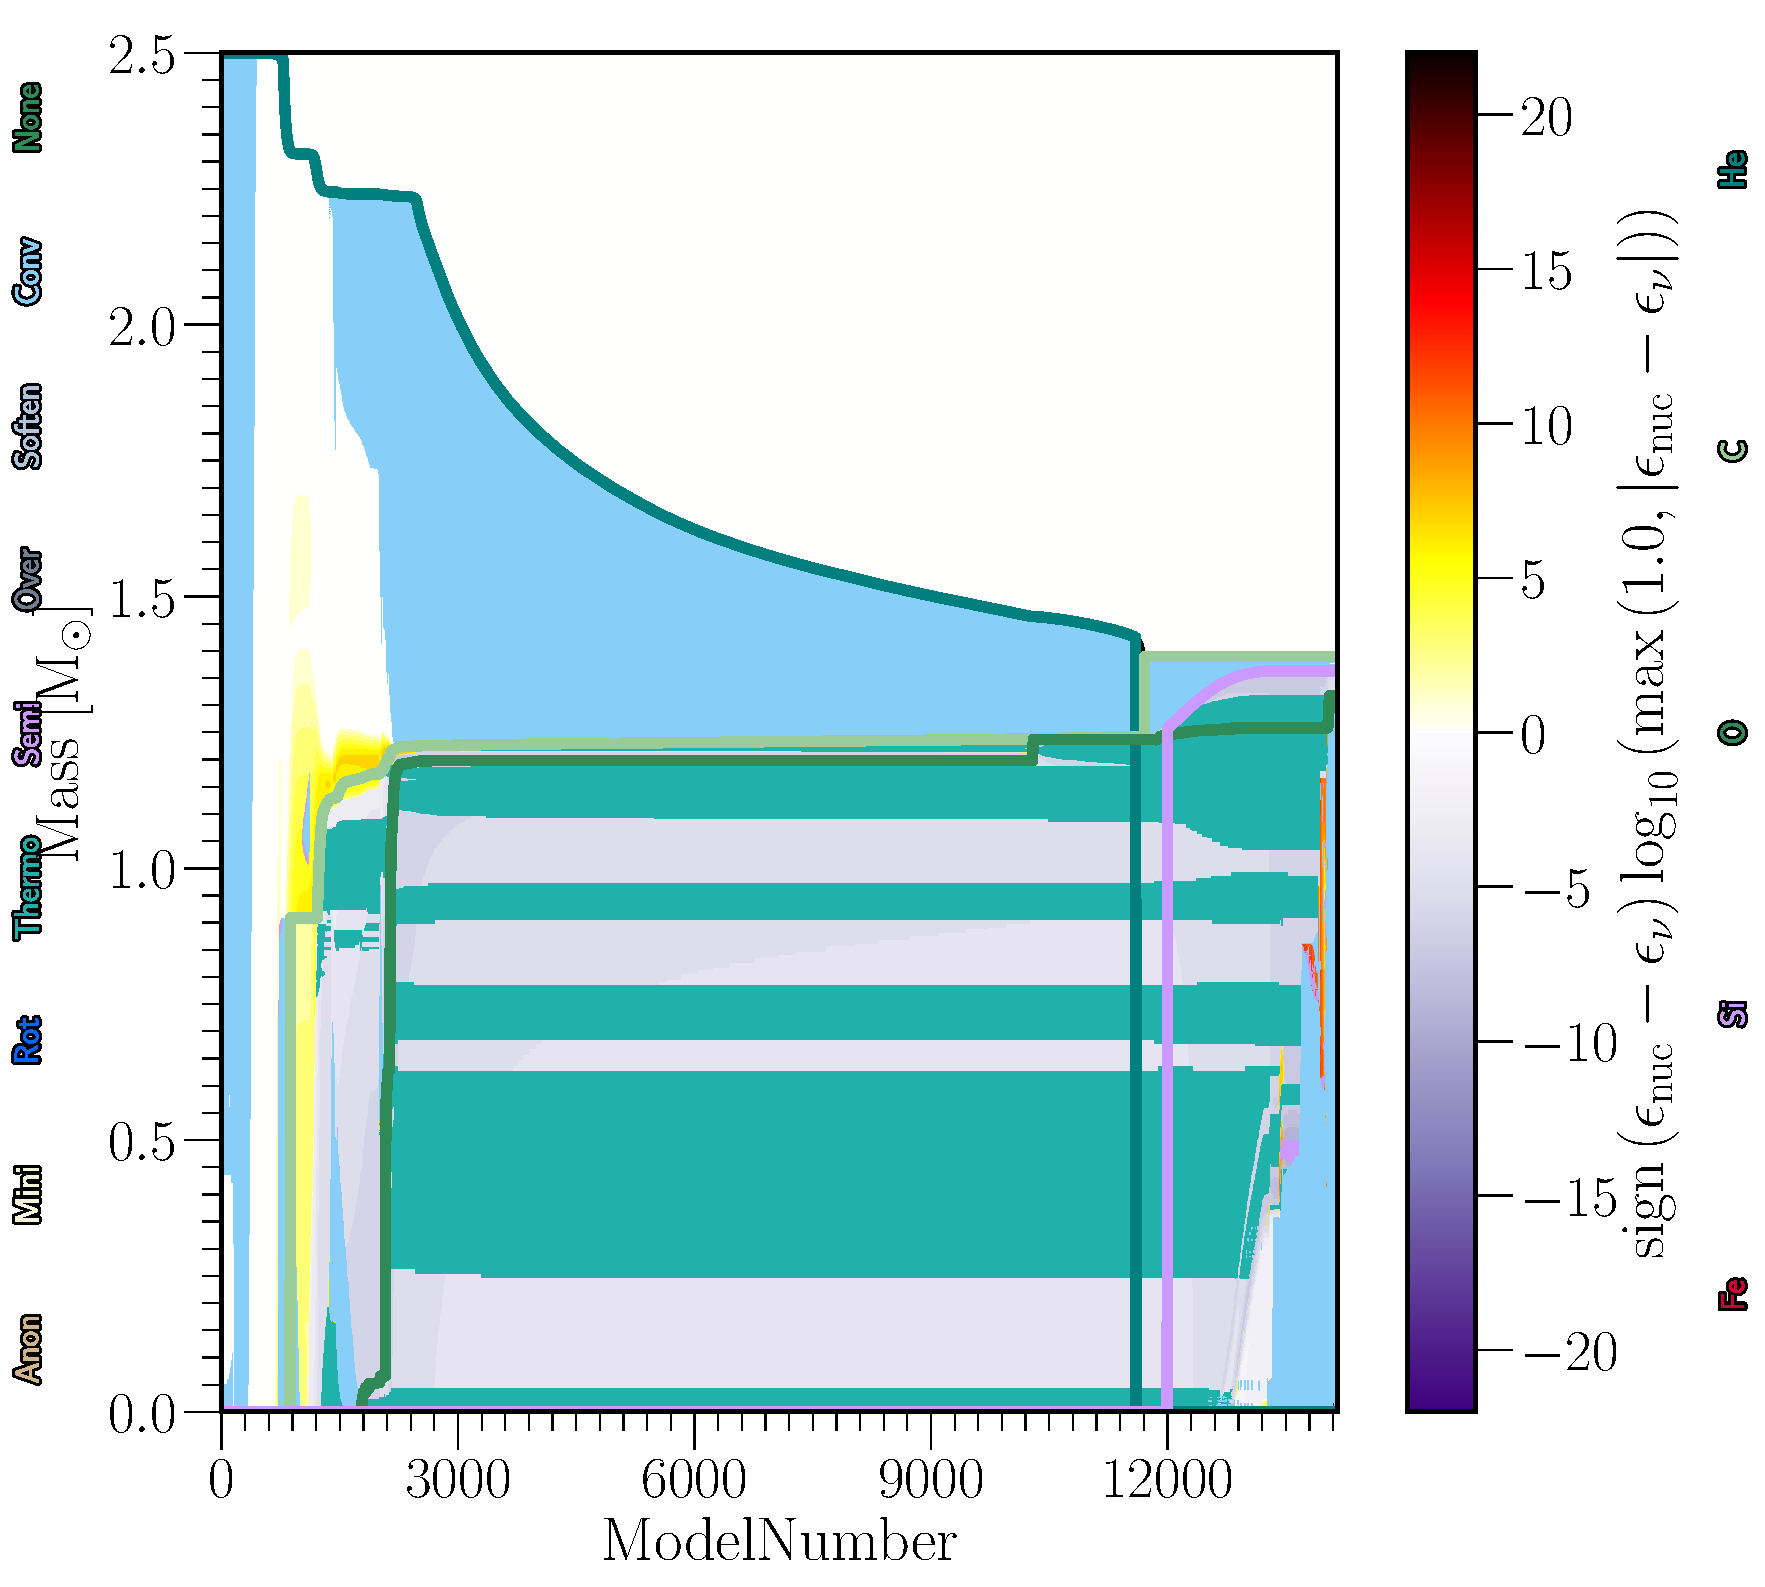
\includegraphics[width=0.5\columnwidth]{../figures/chapter4/Kipp_2p5_0p02_0p0.pdf}
        \caption{Kippenhahn diagram of the $2.5 \rm M_{\odot}$ helium star with $Z = 0.02$ and no overshooting that leads to the final structure shown in Figure \ref{fig:abun_c}. Blue areas denote regions with convection; green-coloured areas indicate thermohaline mixing. The intensity shown in the colour-bar, indicates the net energy-production rate. During electron captures on $\rm ^{24}Mg$ and subsequent carbon burning, the core becomes convective.}
        \label{fig:Kipp}
    \end{figure}
    
    
    The core of our stellar models in the mass range $\rm M_i = 1.8 - 2.7 \ M_{\odot}$ grow to near Chandrasekhar masses due to helium shell-burning, and reach a plateau of $\rm M_c \sim 1.36 \pm 0.01 \ M_{\odot}$ whilst the extended He-rich envelope is easily ejected via a strong wind (see section \ref{sec:wind} for discussion).
    Subsequently, the existing carbon in the core ignites initiating convective motions that feed the core with more carbon, and the star enters a short carbon burning phase. The energy yield from carbon burning is sufficient to raise the temperature for explosive oxygen burning under extreme degenerate conditions to occur. As a result, a thermal runaway ensues and the star which contains no helium at the time of the explosion, it would be observable, most likely, as a SN\,Ia.
    
    Convective overshooting leads to larger convective cores which, naturally, prolongs the time the star spends in the helium main-sequence phase and thus, lengthens its total lifetime. The reason is that an enlarged convective zone will supply the helium burning core with more fuel. The additional fuel will affect the rate at which nuclear energy is released, thus we expect higher luminosity in the cases where convective overshoot mixing is included. Moreover, the increased size of the metal core will shift the mass range for which we observe the behaviour described above, to lower initial masses. This shifting in the initial mass range caused by the overshoot mixing and the metallicity is more evident and easily understood in Figure\, \ref{fig:parameterSpace} where we display the full parameter space in a raster format. The color of each pixel indicates the composition of the star at the time the evolution was terminated. Hatched regions represent models that have develop a near-Chandrasekhar mass core whilst, at the same time, most of their envelope has been stripped away. Thus, these are all candidates for undergoing a late thermal runaway, avoiding this was an electron-capture induced implosion. However, we were not able to evolve all of those models up to the point of explosive burning, so we could not accurately constrain the minimum mass fraction of carbon required for such an outcome. It might be the case for some ONe cores in the high end of this mass-range, that the amount of residual carbon is too small to initiate an oxygen deflagration at low densities, and the star will still, most likely, evolve towards an ECSN. Similarly, ONe cores at the lower end of this mass-range could still end up as massive ONe WDs if they don't survive the Urca cooling phase (see below). In this case, the ONe WDs would have a small amount of carbon distributed in their cores.
    
    % Since all models with an ONe structure (green pixels) grow to near Chandrasekhar masses, they will undergo thermal runaway as a result of the remaining carbon in their cores, avoiding this way to end up as massive oxygen-neon white dwarfs or ECSN. 
    
   \begin{figure*}[ht]
        \centering
        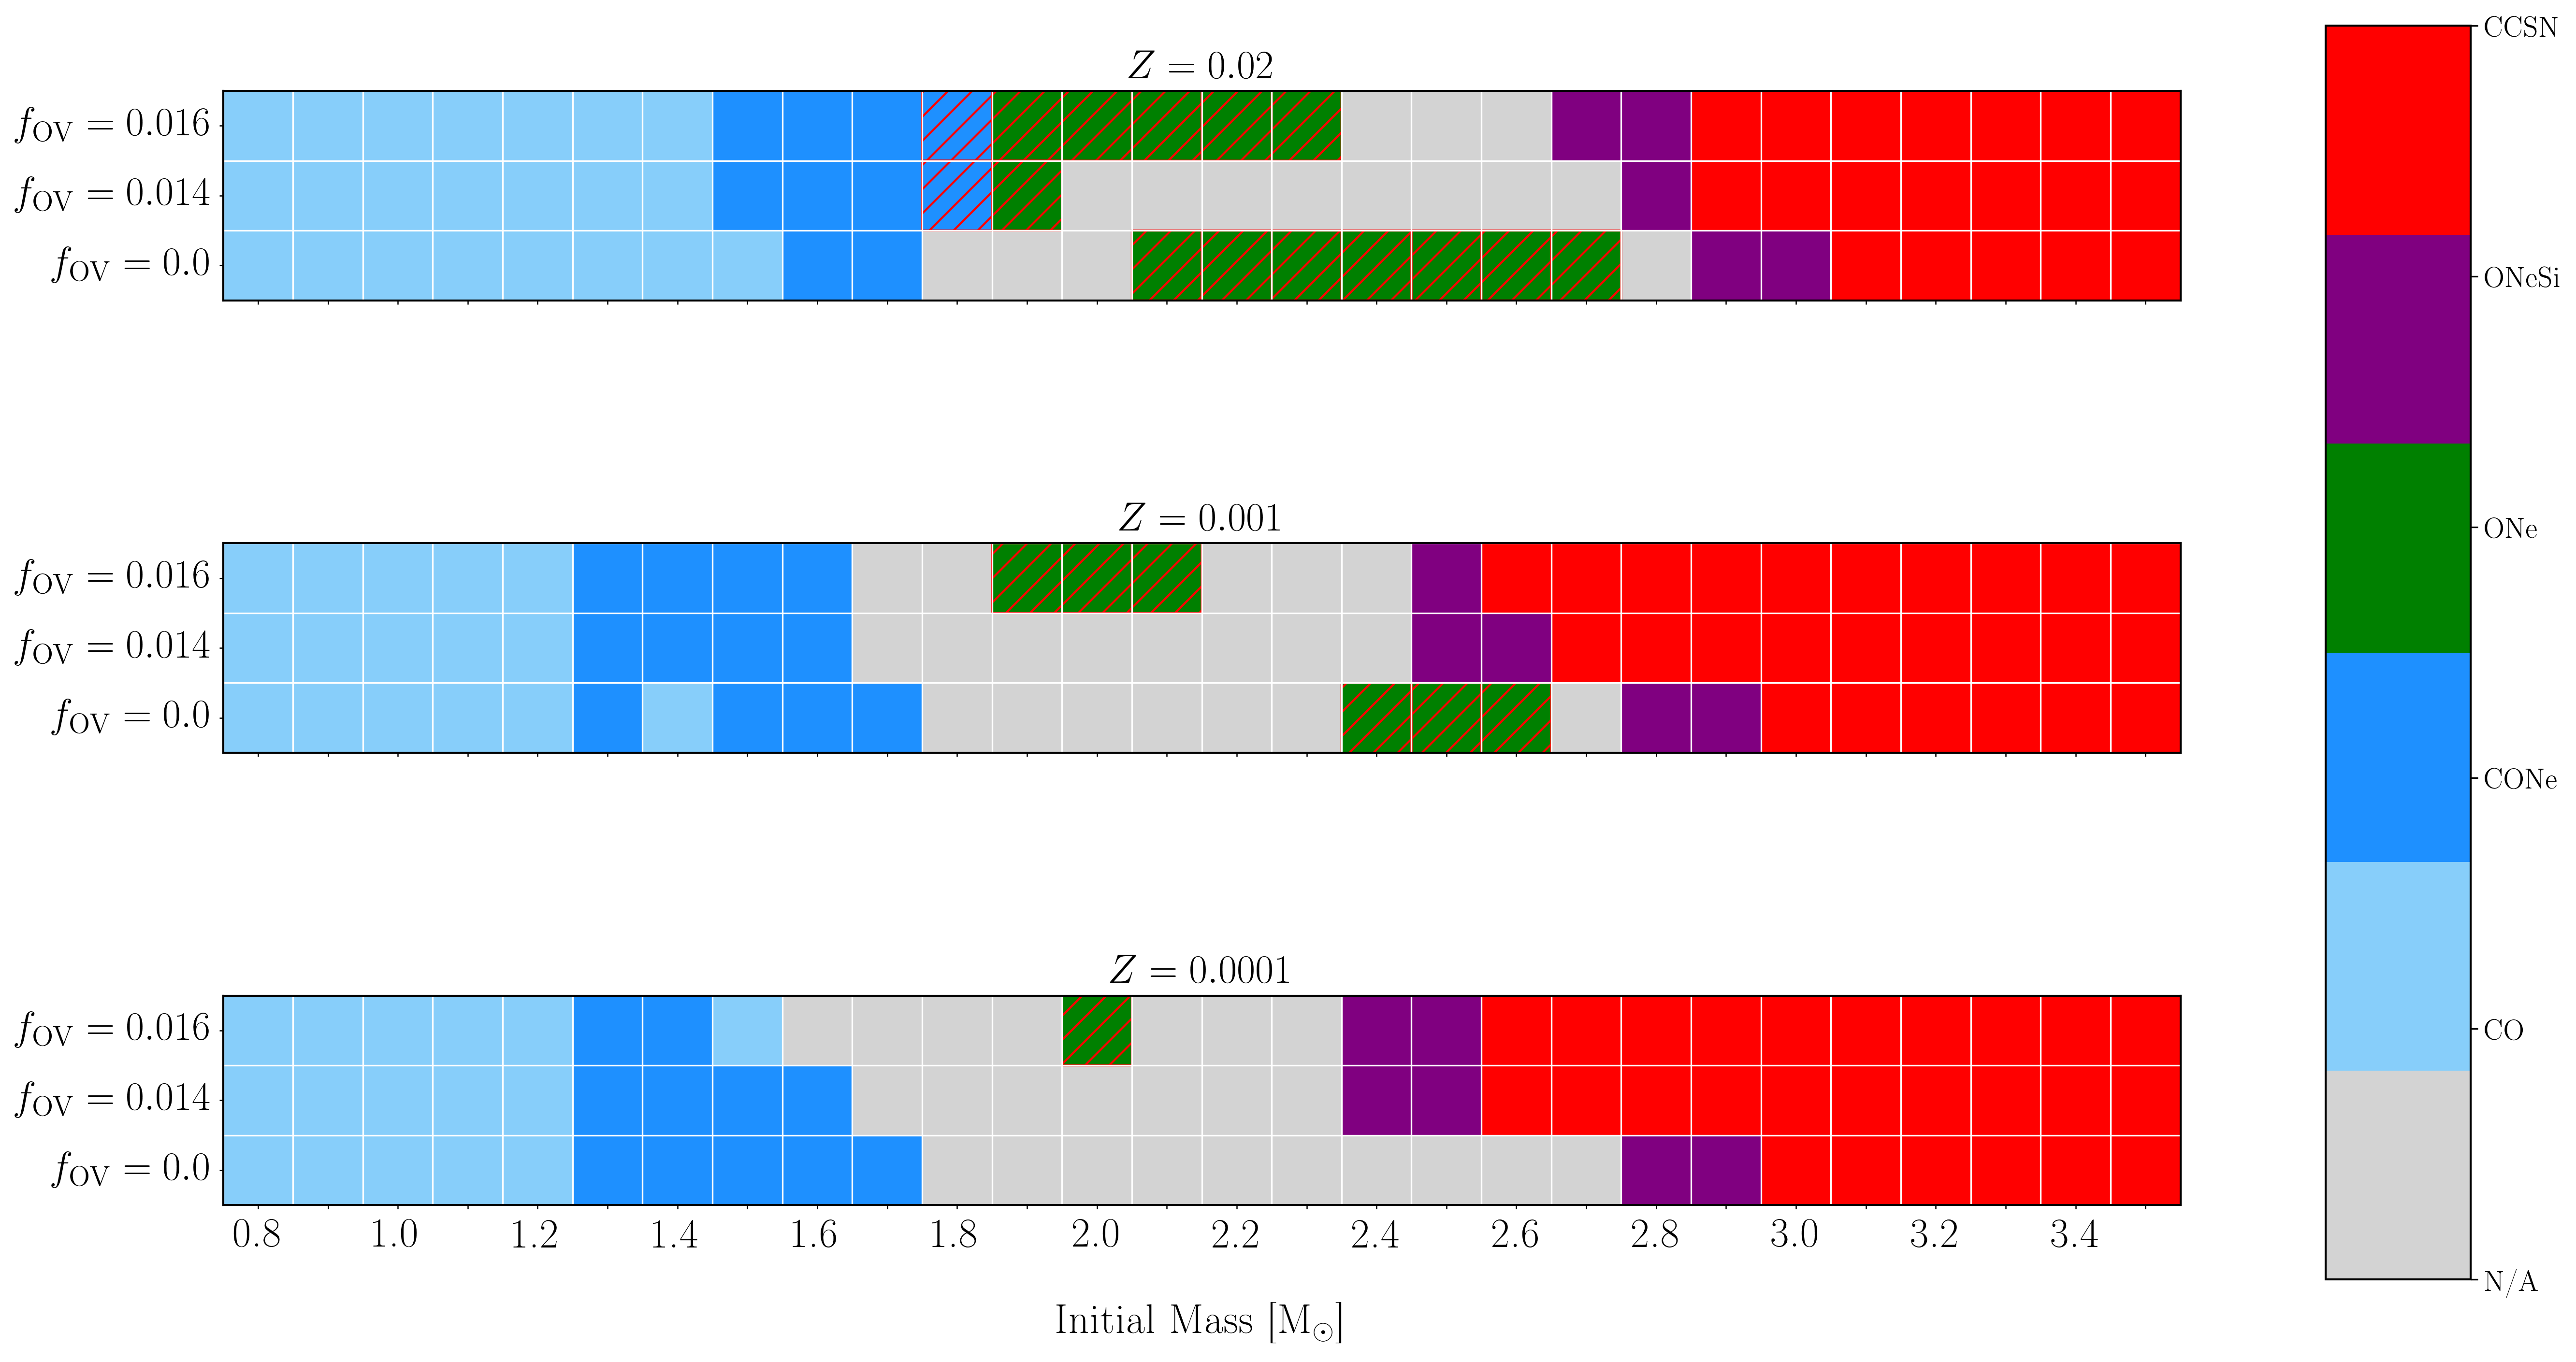
\includegraphics[width=0.8\textwidth]{../figures/chapter4/parameterSpaceRaster.png}
        \caption{Full parameter space in raster format. Metallicity for the bottom, middle, and top panel is $Z=0.0001$, $Z=0.001$, and $Z=0.02$ respectively, whilst the color-bar indicates the composition of the model at the moment our simulation was terminated. Hatched regions show models that have developed a core mass in the range $1.35$ - $1.37$ M$_{\odot}$, and can experience a thermonuclear runaway (see text for caveat).}
        \label{fig:parameterSpace}
    \end{figure*}
    
    On the other hand, metallicity seems to adversely affect core growth. The effects of overshooting and metallicity on core growth can be also seen in Figure\, \ref{fig:coreGrowth} which shows the final core mass of our stellar models as a function of the initial mass. Missing data points correspond to models for which the code crashed before they were able to get rid of their helium envelope, thus we couldn't follow the evolution past the hot bottom burning phase and obtain a reliable estimate for the final core mass. The scattering that appears at the high-end of our grid is most likely due to the fact that these models stopped at different evolutionary stages; nonetheless, in all of those cases, the core mass has either exceeded the Chandrasekhar mass limit, or the star has developed an ONeSi structure that will eventually lead to a core-collapse, rendering these models irrelevant to our work.
    

    \begin{figure*}[ht!]
        \centering$
        \begin{array}{cc}
        	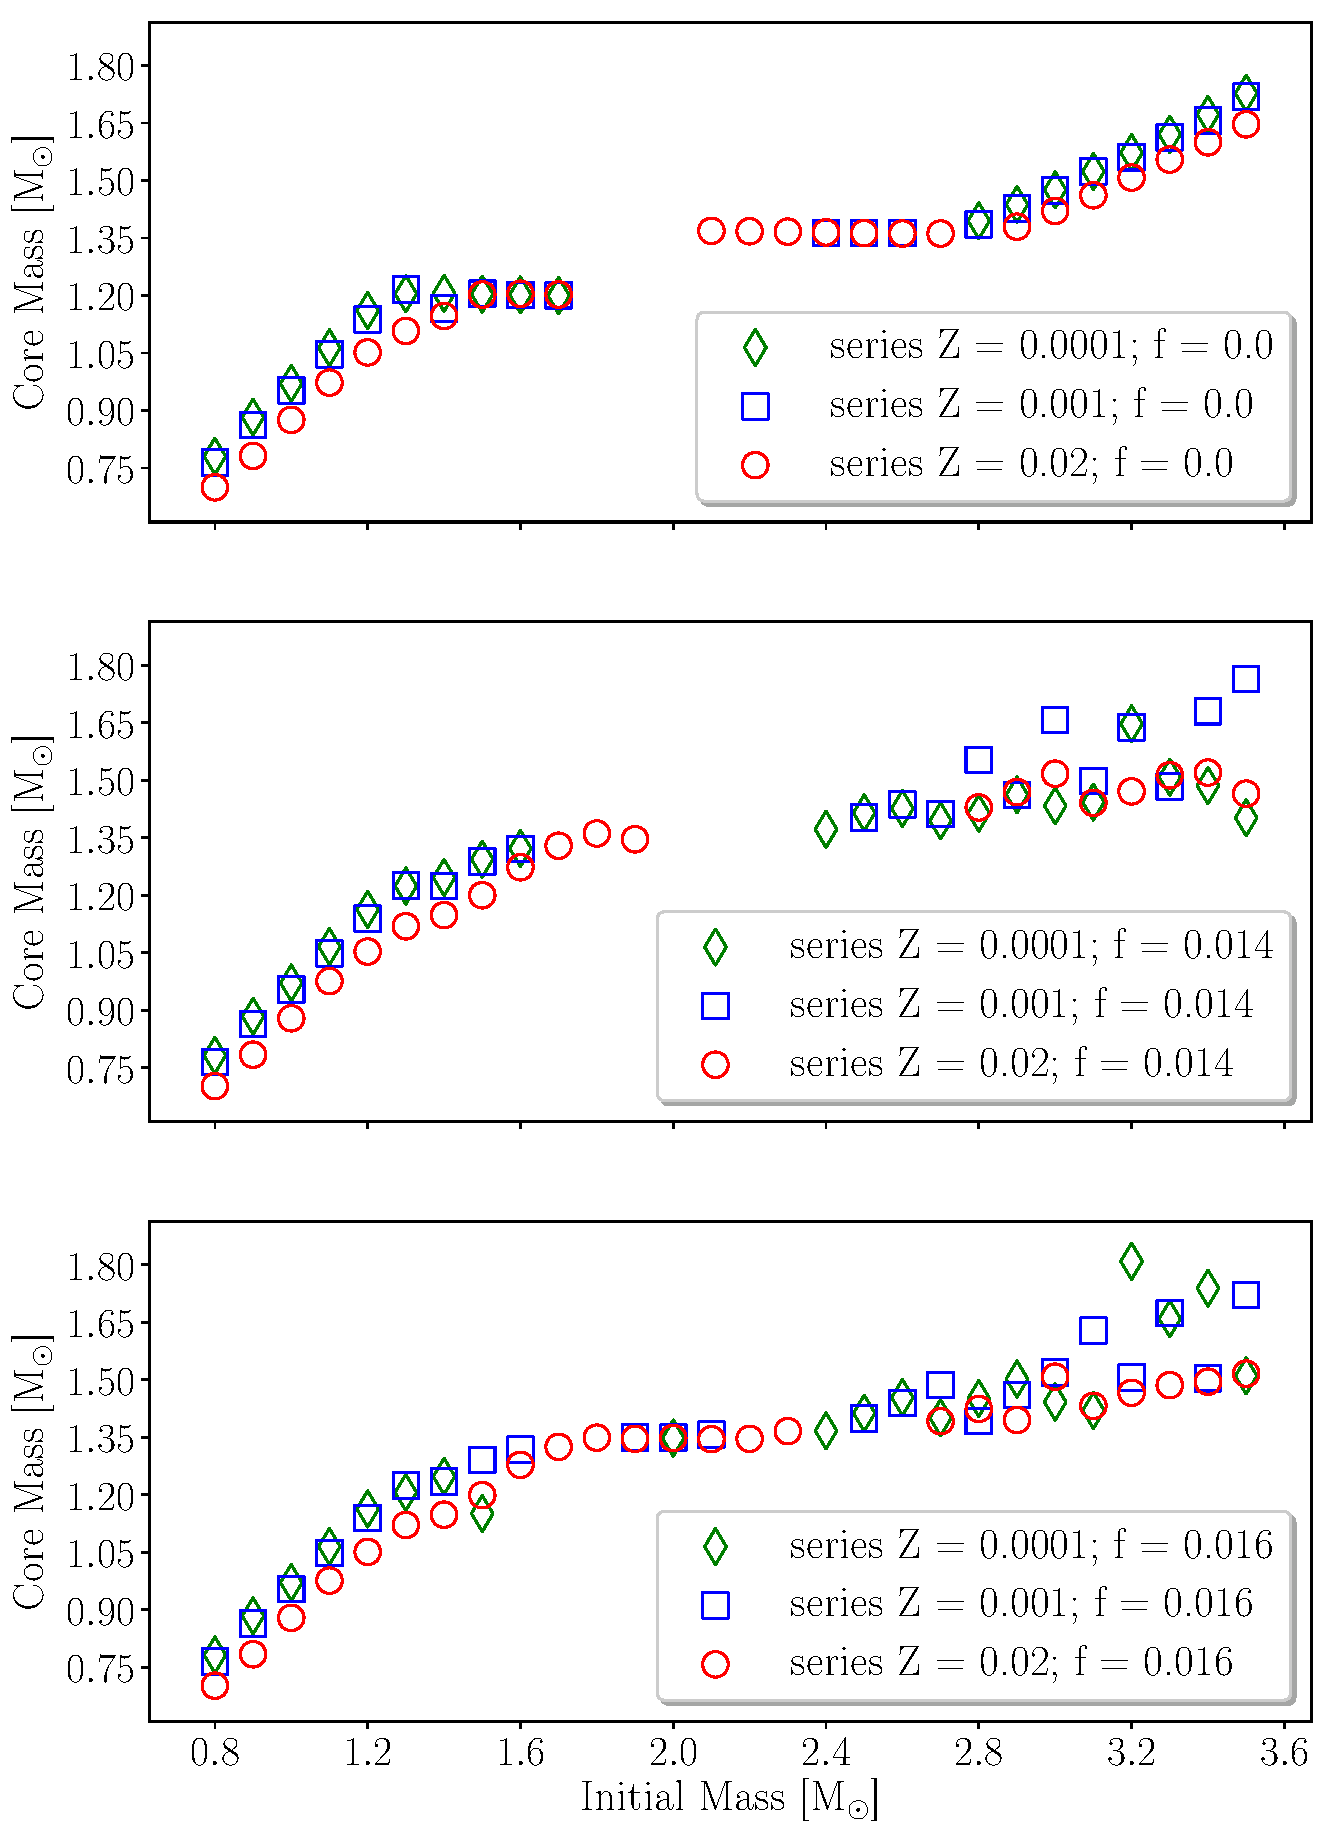
\includegraphics[width=0.45\textwidth]{../figures/chapter4/coreGrowth_merge1.pdf} &
        	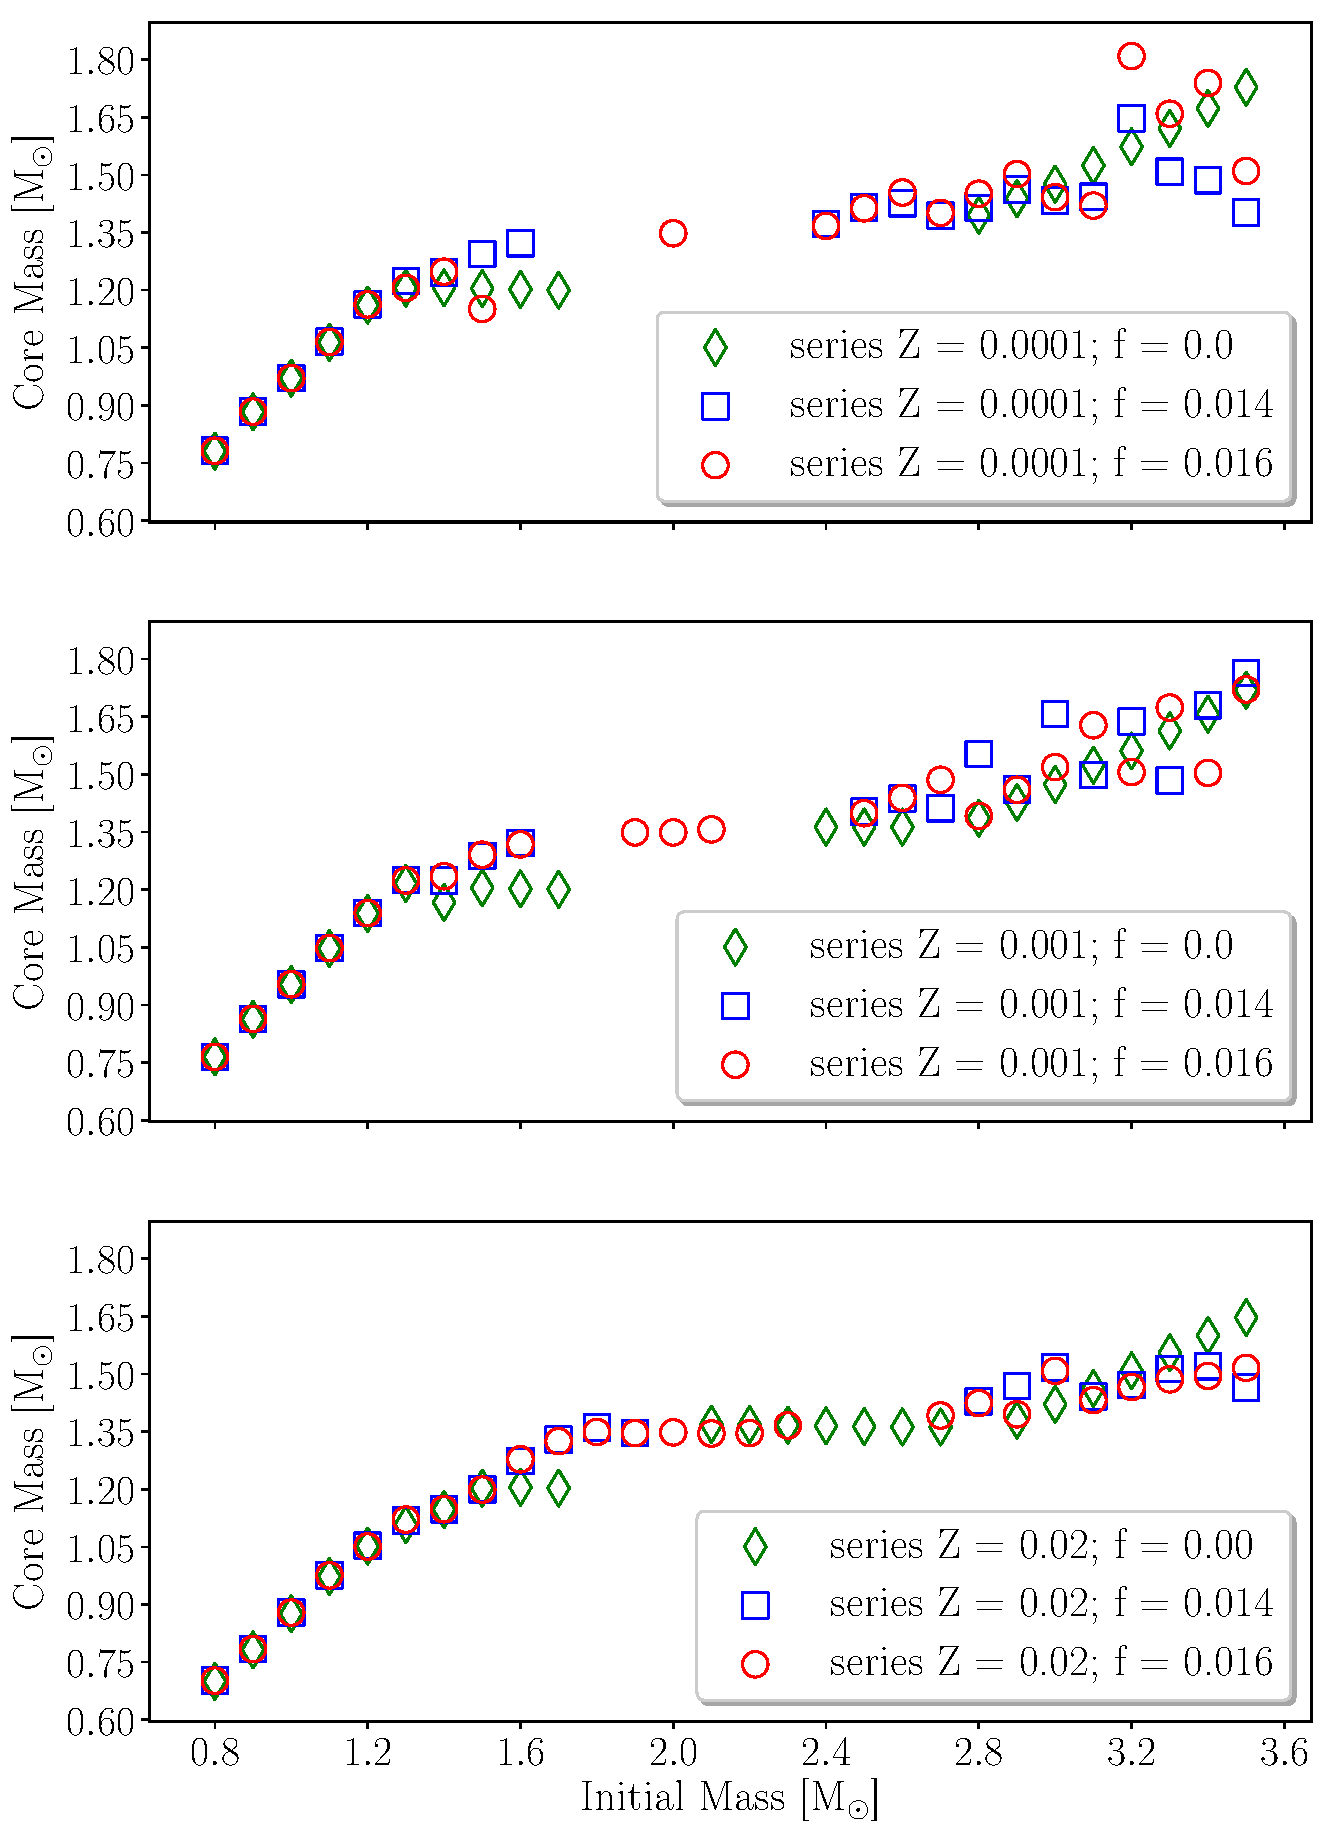
\includegraphics[width=0.45\textwidth]{../figures/chapter4/coreGrowth_merge2.pdf} \\
        \end{array}$
        \caption{Core growth for different metallicity environments (left), and overshooting factors (right). Models that experience thermal runaway develop a core of $M_c \sim 1.36 \pm 0.01$ M$_{\odot}$ (plateau) due to He-shell burning. Missing data points correspond to models which their evolution ended abruptly, hence their final core mass could not be estimated.}
        \label{fig:coreGrowth}
    \end{figure*}
    
    
% -----------------------------------------------------------
%%                  RESULTS 3
% -----------------------------------------------------------
    \subsection{Wind and Envelope Ejection} \label{sec:wind}
%%% goetz
There are two phases where mass loss through stellar winds can affect the outcome of our model computations. Firstly, because of its long duration, mass-loss in the core helium-burning phase has the potential to reduce the stellar mass, and thus its core size. In our current models the total mass removed in this phase is of the order of 0.1\,$\rm M_\odot$, and its influence on our results is negligible. Secondly, our models reach very high luminosities towards the end of their evolution where the stars are much cooler (up to $\rm \log{L/L_\odot = 6.25}$ for the example in Figure\, \ref{fig:HRD}). In this short phase the remaining He-envelope is removed, which is crucial for the formation of type-Ia SNe in our scenario. For our scenario it is required that that the mass-loss rates in the core He-burning phase are small enough to let the core grow, and that they are high enough in the cool evolved phase to remove the remaining He envelope.

   % HRD placeholder
    \begin{figure}[h!]
        \centering
        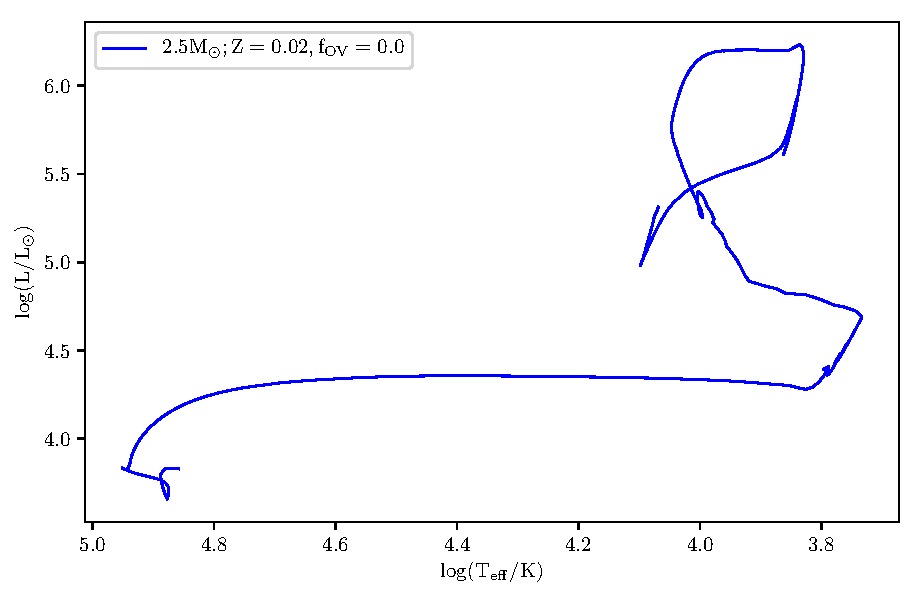
\includegraphics[width=0.6\columnwidth]{../figures/chapter4/HRD.pdf}
        \caption{HR diagram for the $\rm 2.5 \ M_{\odot}$ fiducial model, starting from helium main sequence phase.}
        \label{fig:HRD}
    \end{figure}


In our models we adopt the ``\texttt{Dutch}" \mesa wind scheme which extrapolates empirical mass-loss relations for more massive Wolf-Rayet (WR) stars from \cite{Nugis2000} for $\rm T_{\text{eff}} > 10^4$ K and uses the prescription of \cite{deJager1988} for cool stars. These mass-loss rates are very uncertain. Empirically, the mass-loss properties of low-mass He-stars in the range of our models are still very uncertain, mainly because they are only formed in binary systems where they are difficult to observe \citep{Smith2017,Zapartas2017}. Recent theoretical works suggest that the mass-loss rates of low-mass helium stars could lie significantly below the relations for massive WR stars \citep{Graefener2017,Vink2017}. This means that the mass-loss rates in the core helium burning phase are most likely small enough to allow our scenario to work.
        
In late phases, when the degenerate core is near its maximum mass, our models reach extremely high super-Eddington luminosities up to $\rm \log{L/L_\odot = 6.25}$), resulting in a strong stellar wind that eventually removes the He-rich envelope. While the mass-loss rates of cool stars in this regime are also extremely uncertain, it is notable that the maximum values in our models lie in a plausible range near the theoretically expected maximum values for super-Eddington winds \citep[][]{Owocki:2004zz,Smith2006}.
        
 



% -----------------------------------------------------------
%%                  RESULTS 4
% -----------------------------------------------------------
    \subsection{The Role of Residual Carbon} \label{sec:residualCarbon}
    
        \subsubsection{Oxygen-Neon Cores}
        
        As the core is compressed, compressional heating will eventually balance thermal neutrino emission. The core then will continue to compress and heat up until its density reaches the threshold value of various Urca pairs. The $\rm ^{25}Mg$ - $\rm ^{25}Na$, and $\rm ^{23}Na$ - $\rm ^{23}Ne$ pairs are of utmost importance in our case, and occur at densities $\rm \log(\rho_c / \rm gr \ cm^{-3}) \approx 9.1$, and $\rm \log(\rho_c / \rm gr \ cm^{-3}) \approx 9.2$ respectively. \cite{Tsuruta1970} have shown that the energy loss rate via Urca-cooling depends on the fourth power of temperature ($\rm \propto T^4$), hence this effect is more prominent in our hot, young ONe cores rather than in cooled WDs.
        
        The effect of Urca-cooling can be seen in Figure\, \ref{fig:RhoT} where the evolution of our fiducial stellar model with initial mass of $2.5 \rm \  M_{\odot}$, and solar metallicity is being displayed (blue line). The density at which carbon is ignited is illustrated with a dotted black line, taken from \mesa; however, \mesa assumes a 100\% composition of carbon and thus, the limits shown in Figure\, \ref{fig:RhoT} are only approximated. In our models, Urca-cooling occurs before central density reaches the threshold for carbon ignition, effectively shifting this stage to higher densities by delaying the ignition of carbon, and altering the nucleosynthetic signature of the explosion. 
        
        Following the Urca cooling phase, there is no significant neutrino emission and the core evolves along the adiabatic curve of Figure\, \ref{fig:RhoT}. Further compression leads to exothermic e-captures on $\rm ^{24}Mg$ nuclei at $\rm \log(\rho_c/gr \ cm^{-3}) \approx 9.6$. The generated heat ignites the residual carbon in a very localized manner due to the sensitivity of carbon reaction rates to temperature. This can be seen as a saw-tooth feature in Figure\, \ref{fig:RhoT}, where heating from carbon burning antagonizes neutrino cooling. We did not investigate the effect of $\rm ^{24}Mg$ mass fraction, however \cite{Gutierrez2005} have shown that it could play a major role on the subsequent evolution.
        
        The energy yield from carbon burning will eventually lead to dynamical burning of oxygen. \cite{Woosley2004} estimates that the end of the carbon simmering phase occurs roughly at $\rm \log(T_c/ \rm K) \approx 8.9$. In our models, the central temperature at the time the core has reached its maximum compactness is $\rm \log(T_c / \rm K) \approx 8.82$. Some of these stellar properties are summarized in Table \ref{tab:properties}.
        
        \begin{figure*}[ht!]
            \centering
            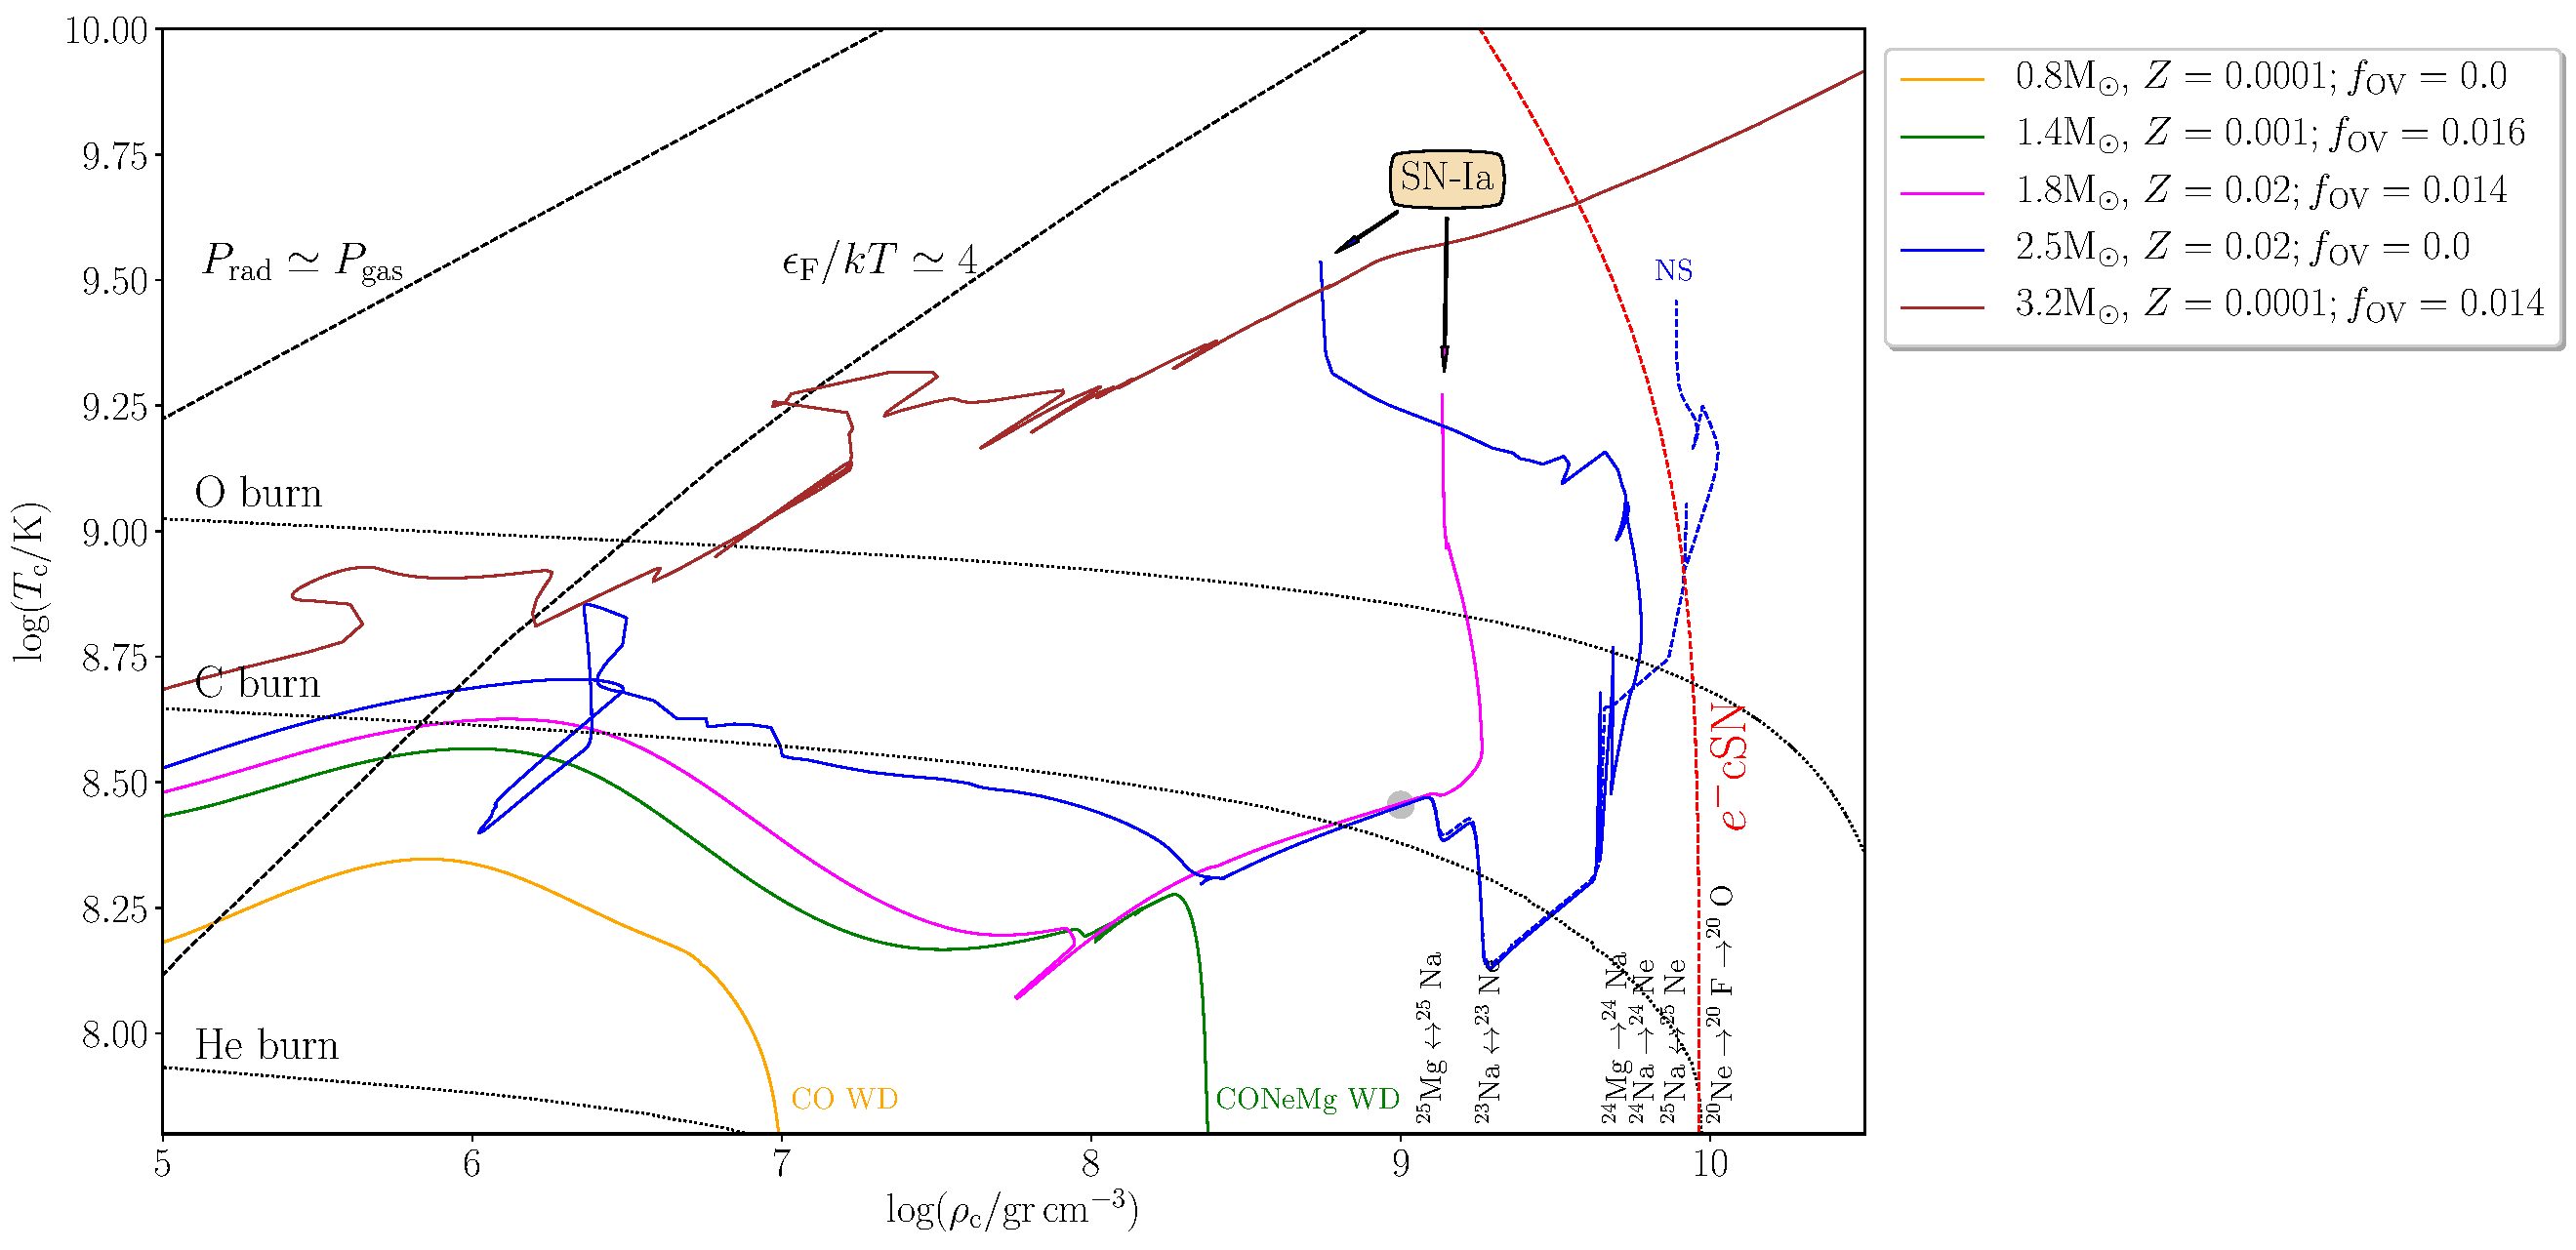
\includegraphics[width=\textwidth]{../figures/chapter4/RhoT.pdf}
            \caption{Examples of the evolution of different initial masses in the $\rm \log(\rho_{\rm c})-\log(T_{\rm c})$ plane. Black dotted lines show approximate ignition curves taken from \mesa. Black dashed lines indicate different pressure regimes whilst the red dashed curve shows the approximate threshold for e-captures on $\rm ^{20}Ne$ nuclei. The blue dashed line refers to the same stellar model as the one with the solid blue line; the only difference is that for the former, all carbon-participating reaction have been switched off leading most likely to an ECSN.}
            \label{fig:RhoT}
        \end{figure*}
        
        In order to mimic a carbon-free core and demonstrate the effects of residual carbon, we evolve a series of models for which we have set the rate of all carbon-participating nuclear reactions to zero, once they reached a central density of $\rm \log(\rho_c / \rm gr \ cm^{-3}) = 9.0$ for the first time (grey circle in Figure\, \ref{fig:RhoT}). The choice of this density value is quite arbitrary since the cores have a ``frozen" carbon profile before the Urca cooling phase. In virtual lack of carbon, the evolution of the core is almost identical to our fiducial model up to the point where electron captures on magnesium occur. From there, compressional heating will once again balance neutrino cooling and the density will continue to grow until it surpasses the threshold for e-captures on $^{20}$Ne nuclei which leads to the ignition of oxygen burning at higher densities. The competition between the propagating oxygen deflagration and e-captures on the post-deflagration nuclear statistical equilibrium (NSE) material will determine the final fate of the star. If the deleptonization of the core due to the electron captures is rapid enough, the core will collapse as a result of pressure support removal. Recently, \cite{Zha2019} found that a deflagration starting from $\log(\rho_c / \rm g \ cm^{-3}) > 10.01$ leads to a collapse, reinforcing our notion that a carbon-free ONe core will, most likely, evolve towards an ECSN and ultimately in the formation of a low-mass neutron star. On the other hand, if the oxygen deflagration triumphs over electron captures, \cite{Jones2016} have shown that a thermonuclear explosion will eject a portion of the degenerate core leaving behind an iron-rich, bound remnant.
        
        
        \subsubsection{Hybrid CONeMg Cores}
    
        A small number of models develop a CO/ONe structure in their core, but still reach the Chandrasekhar limit. We choose a fiducial model of $1.8 \rm M_{\odot}$, with solar metallicity and overshooting ($\rm f_{\rm OV} = 0.014$), in order to demonstrate the evolution of similar structured models. 
        These models ignite carbon and oxygen explosively at even lower densities when compared to the case of non-hybrid stellar models due to the larger mass fraction of carbon they retain.
        
        Since the C-flame does not reach the centre, the Urca pairs $\rm ^{25}Mg$ - $\rm ^{25}Na$, and $\rm ^{23}Na$ - $\rm ^{23}Ne$, which are byproducts of carbon burning, have not produced in abundance. Thus, Urca cooling does not play any major role in the evolution of hybrid cores. In the absence of the aforementioned Urca pairs, once the timescale of compressional heating is equal to the timescale of thermal neutrino emission, the density will continue to raise until the ignition of carbon, and explosive oxygen burning at lower densities ($\rm \log(\rho_c^{\rm ign} / \rm gr \ cm^{-3}) \approx 9.26$) is initiated. The larger amount of carbon could lead to more energetic explosions (magenta line in Figure\, \ref{fig:RhoT}) compared to the case of ONe cores. The central temperature, when density reaches its maximum value, is $\rm \log(T_c / \rm K) \approx 8.58$.
        
        The structure of such hybrid proto-WDs is susceptible to mixing due to their composition gradient (see Figure \ref{fig:abun_a}). As \cite{brooks2017} mention, the ONe mantle has been processed by a carbon burning front that involves several weak reactions, resulting in a lower electron-to-baryon fraction ($\rm Y_e$) with respect to the CO core. This configuration is stable against convection as long as the heavier ONe ashes in the top, are much hotter than the lighter CO bottom. As the temperature gradient is reduced, the core-mantle interface will be subjected to thermocompositional convection and destroyed in a timescale of the order of Kyr, as the WD moves toward an isothermal profile. By the time an explosion can occur, the WD should be well mixed. The same process can re-distribute the residual carbon within ONe cores and reduce it to such levels so a thermal runaway would be unlikely making the AIC a more plausible scenario.

    
 	%\begin{figure*}[ht!]
     %   \centering
     %   \begin{tabular}{cc}
      %  	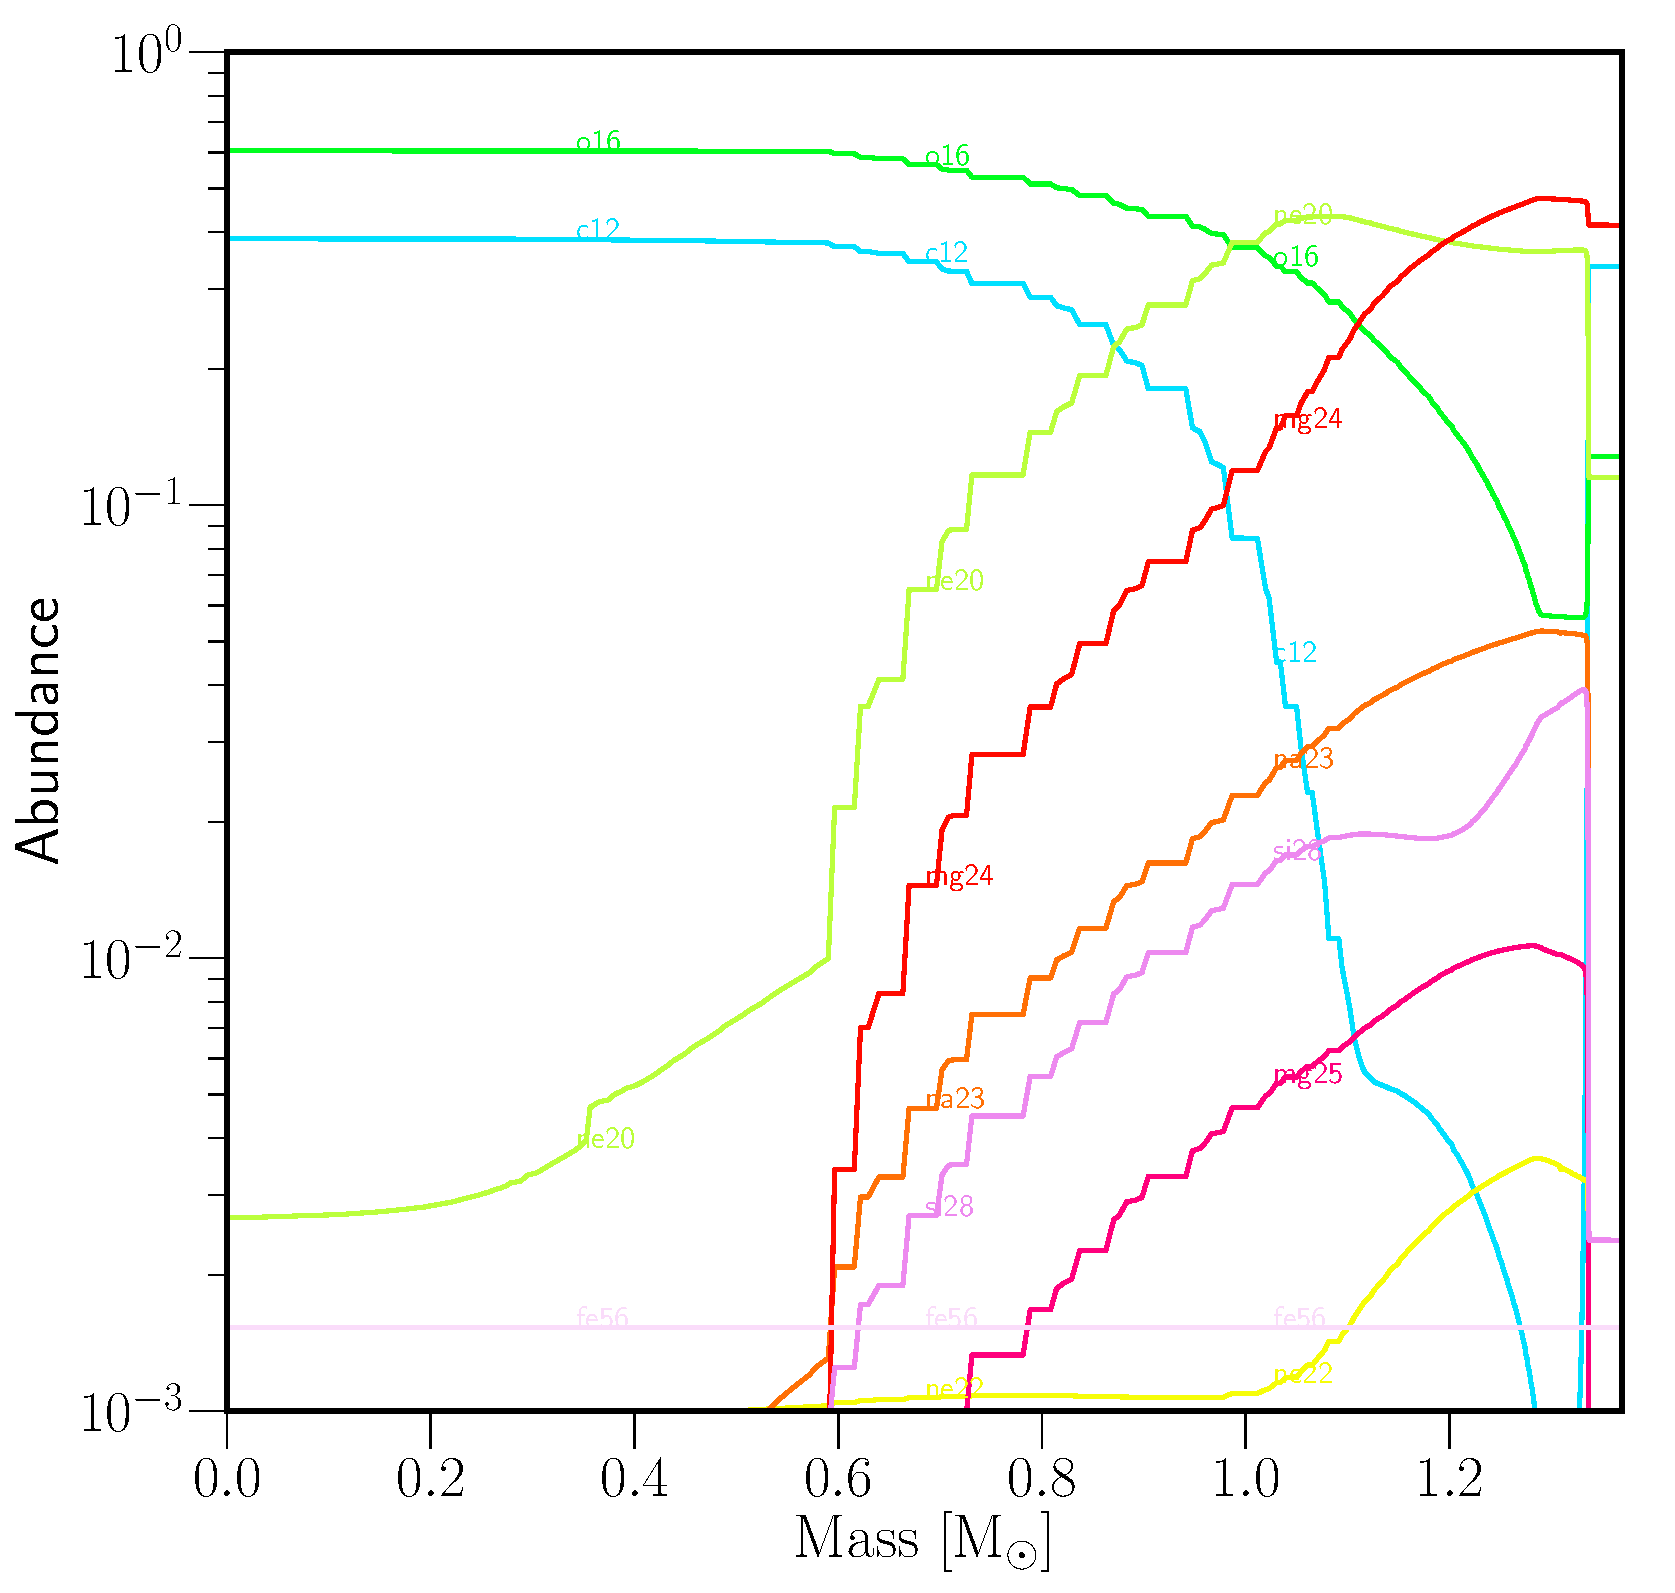
\includegraphics[width=0.45\textwidth]{../figures/chapter4/1p8_logRho9_abun.pdf} &
       % 	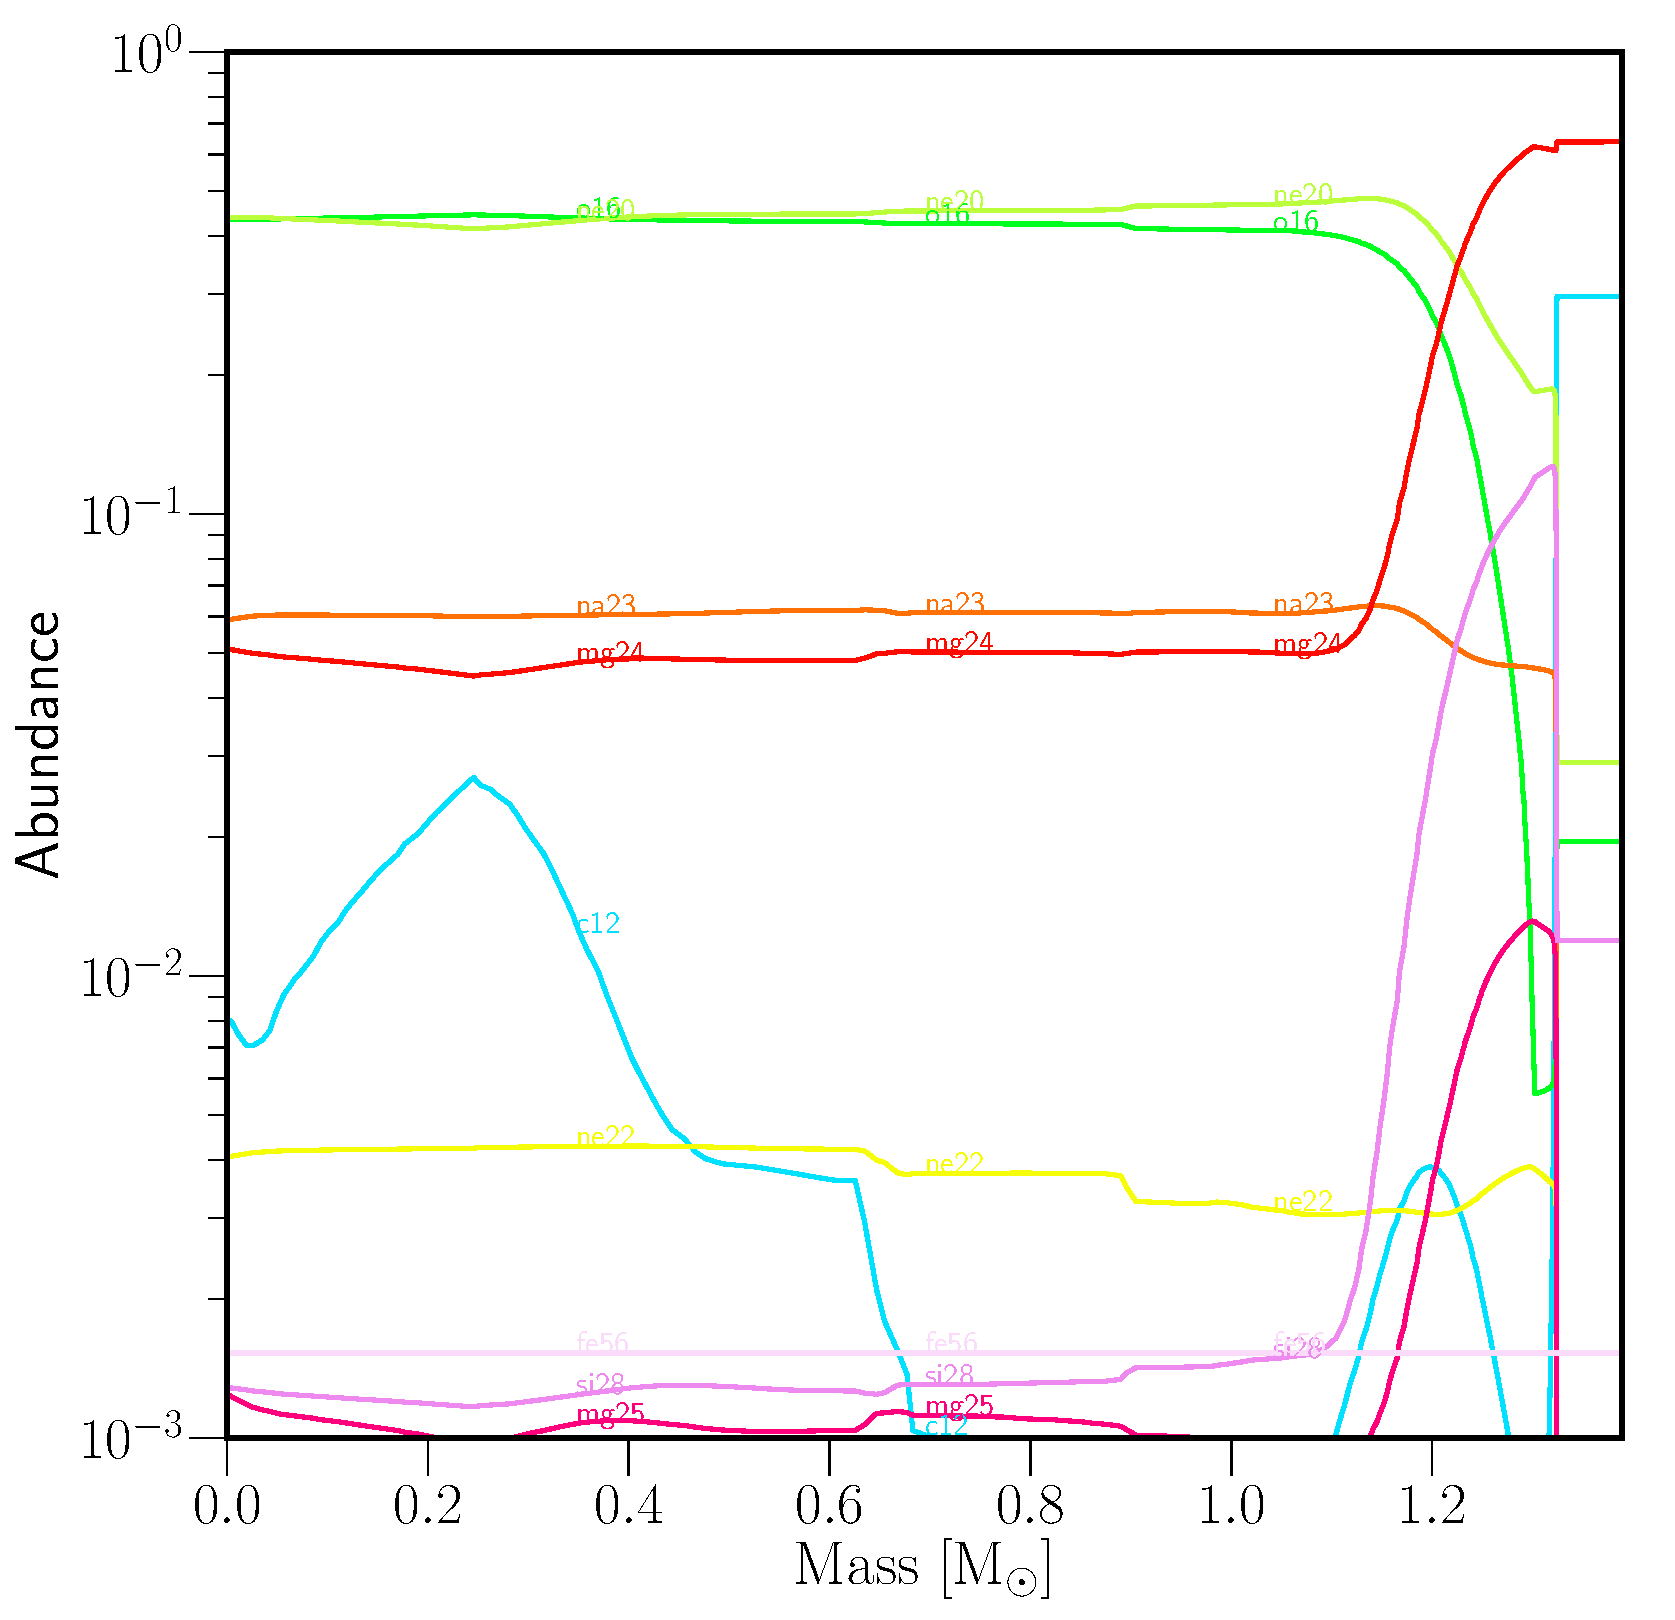
\includegraphics[width=0.45\textwidth]{../figures/chapter4/2p5_logRho_9_abun.pdf} \\
        %	\text{(a) Structure of the $1.8 \rm M_{\odot},  Z=0.02;f_{OV}=0.014$ stellar model, when $\rm \log(\rho_c) = 9.0$ (indicated by the grey circle in Figure \ref{fig:RhoT}).} & \text{(b) Structure of the $2.5 \rm M_{\odot},  Z=0.02;f_{OV}=0.0$ stellar model, when $\rm \log(\rho_c) = 9.0$ (indicated by the grey circle in Figure \ref{fig:RhoT}). Residual carbon from previous burning stages is visible.}\\
        %\end{tabular}
        %\caption{Abundance profiles of our fiducial models during various evolutionary stages.}
        %\label{fig:abundance_profiles}
    %\end{figure*}
    


\begin{figure}
\centering
\begin{subfigure}[b]{.45\linewidth}
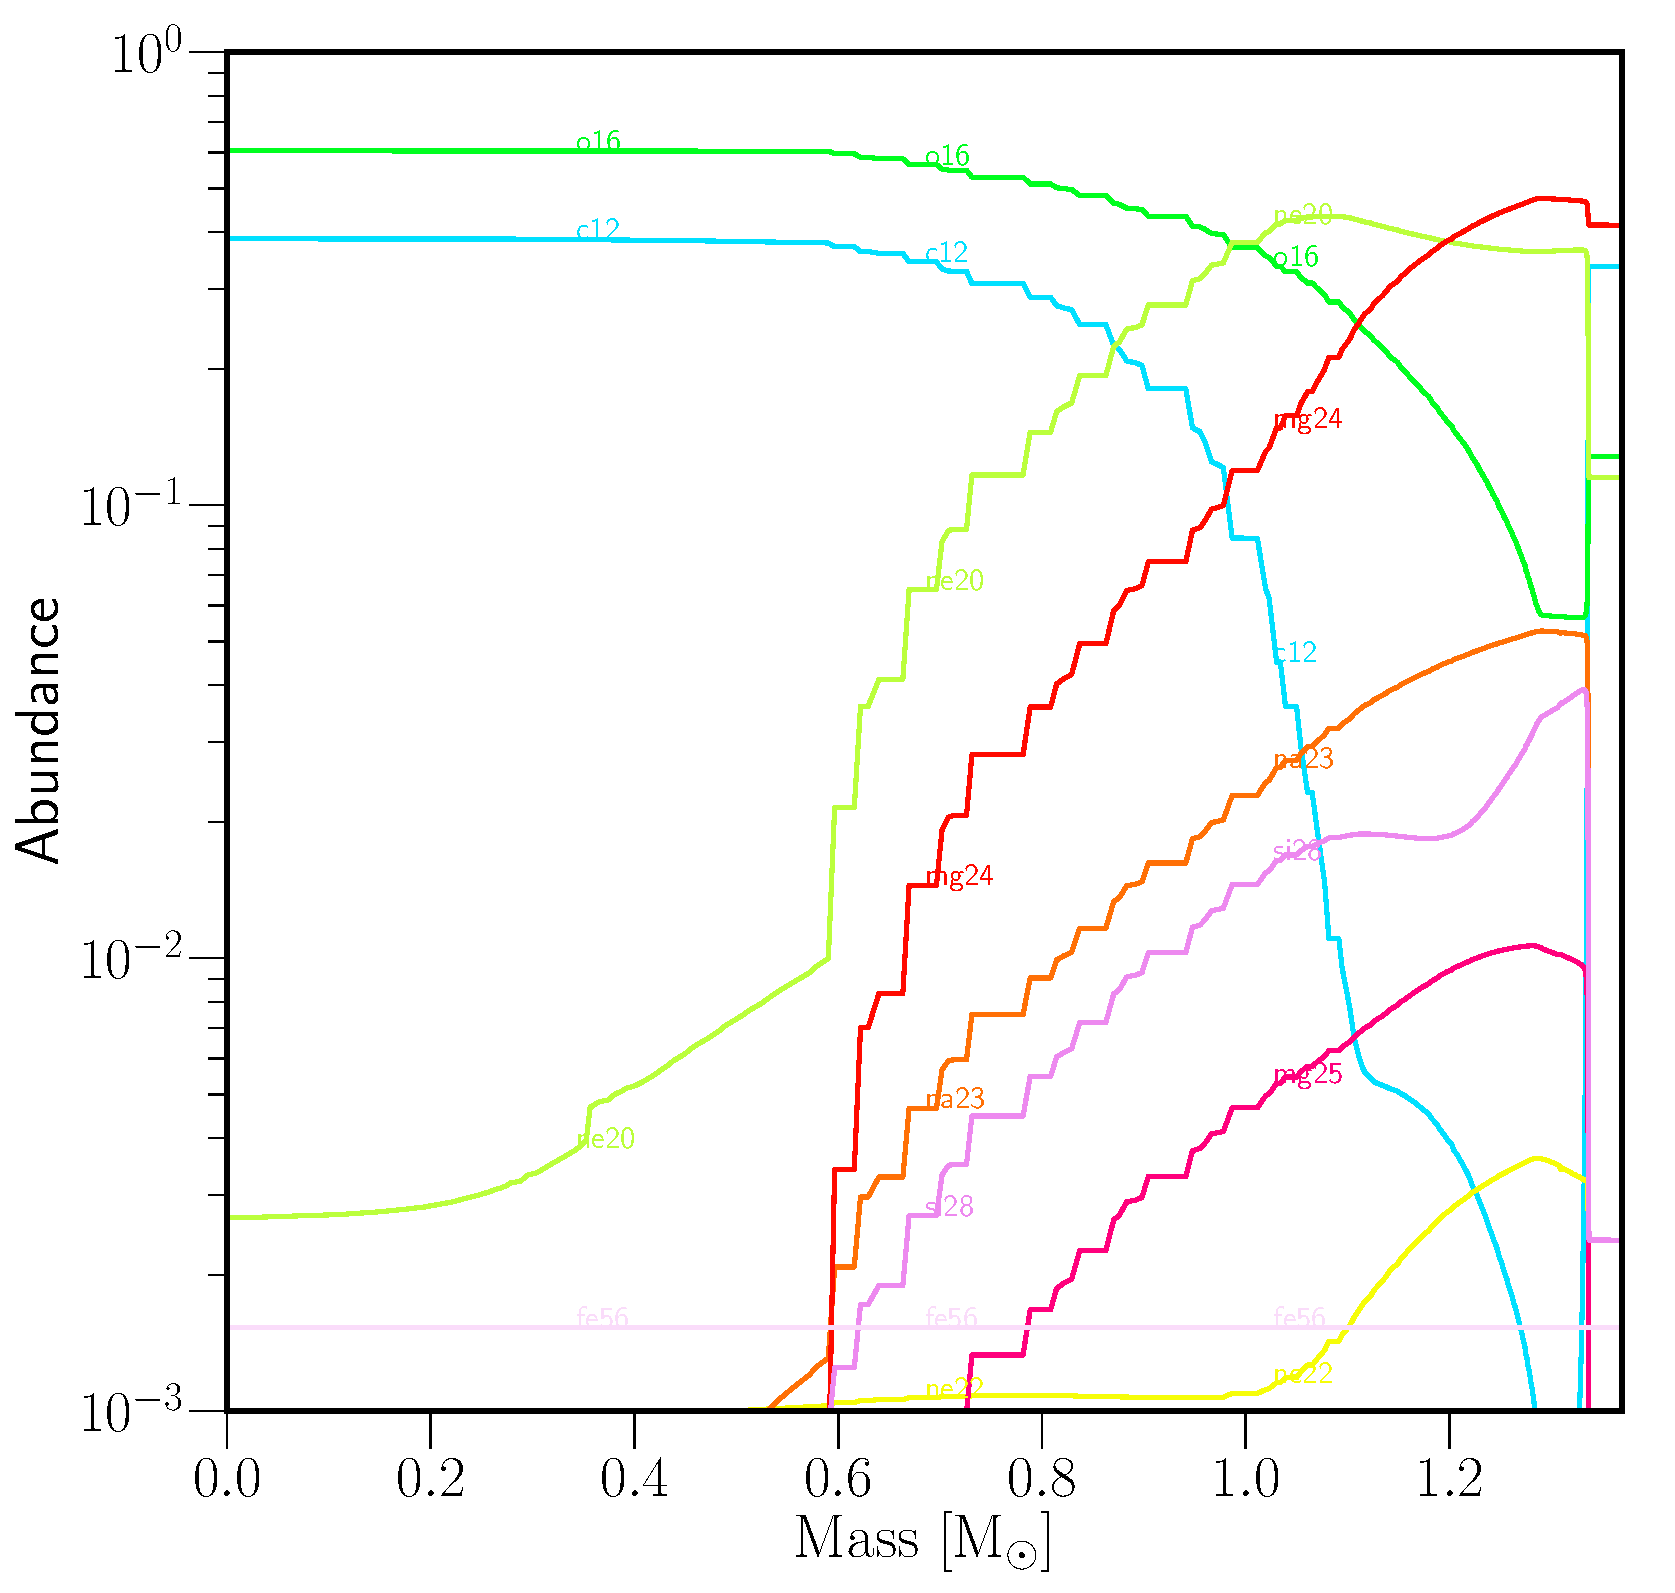
\includegraphics[width=\textwidth]{../figures/chapter4/1p8_logRho9_abun.pdf}
\caption{Structure of the $1.8 \rm \ M_{\odot},  Z=0.02;f_{OV}=0.014$ stellar model.}\label{fig:abun_a}
\hfill
\end{subfigure}
\hfill
\begin{subfigure}[b]{.45\linewidth}
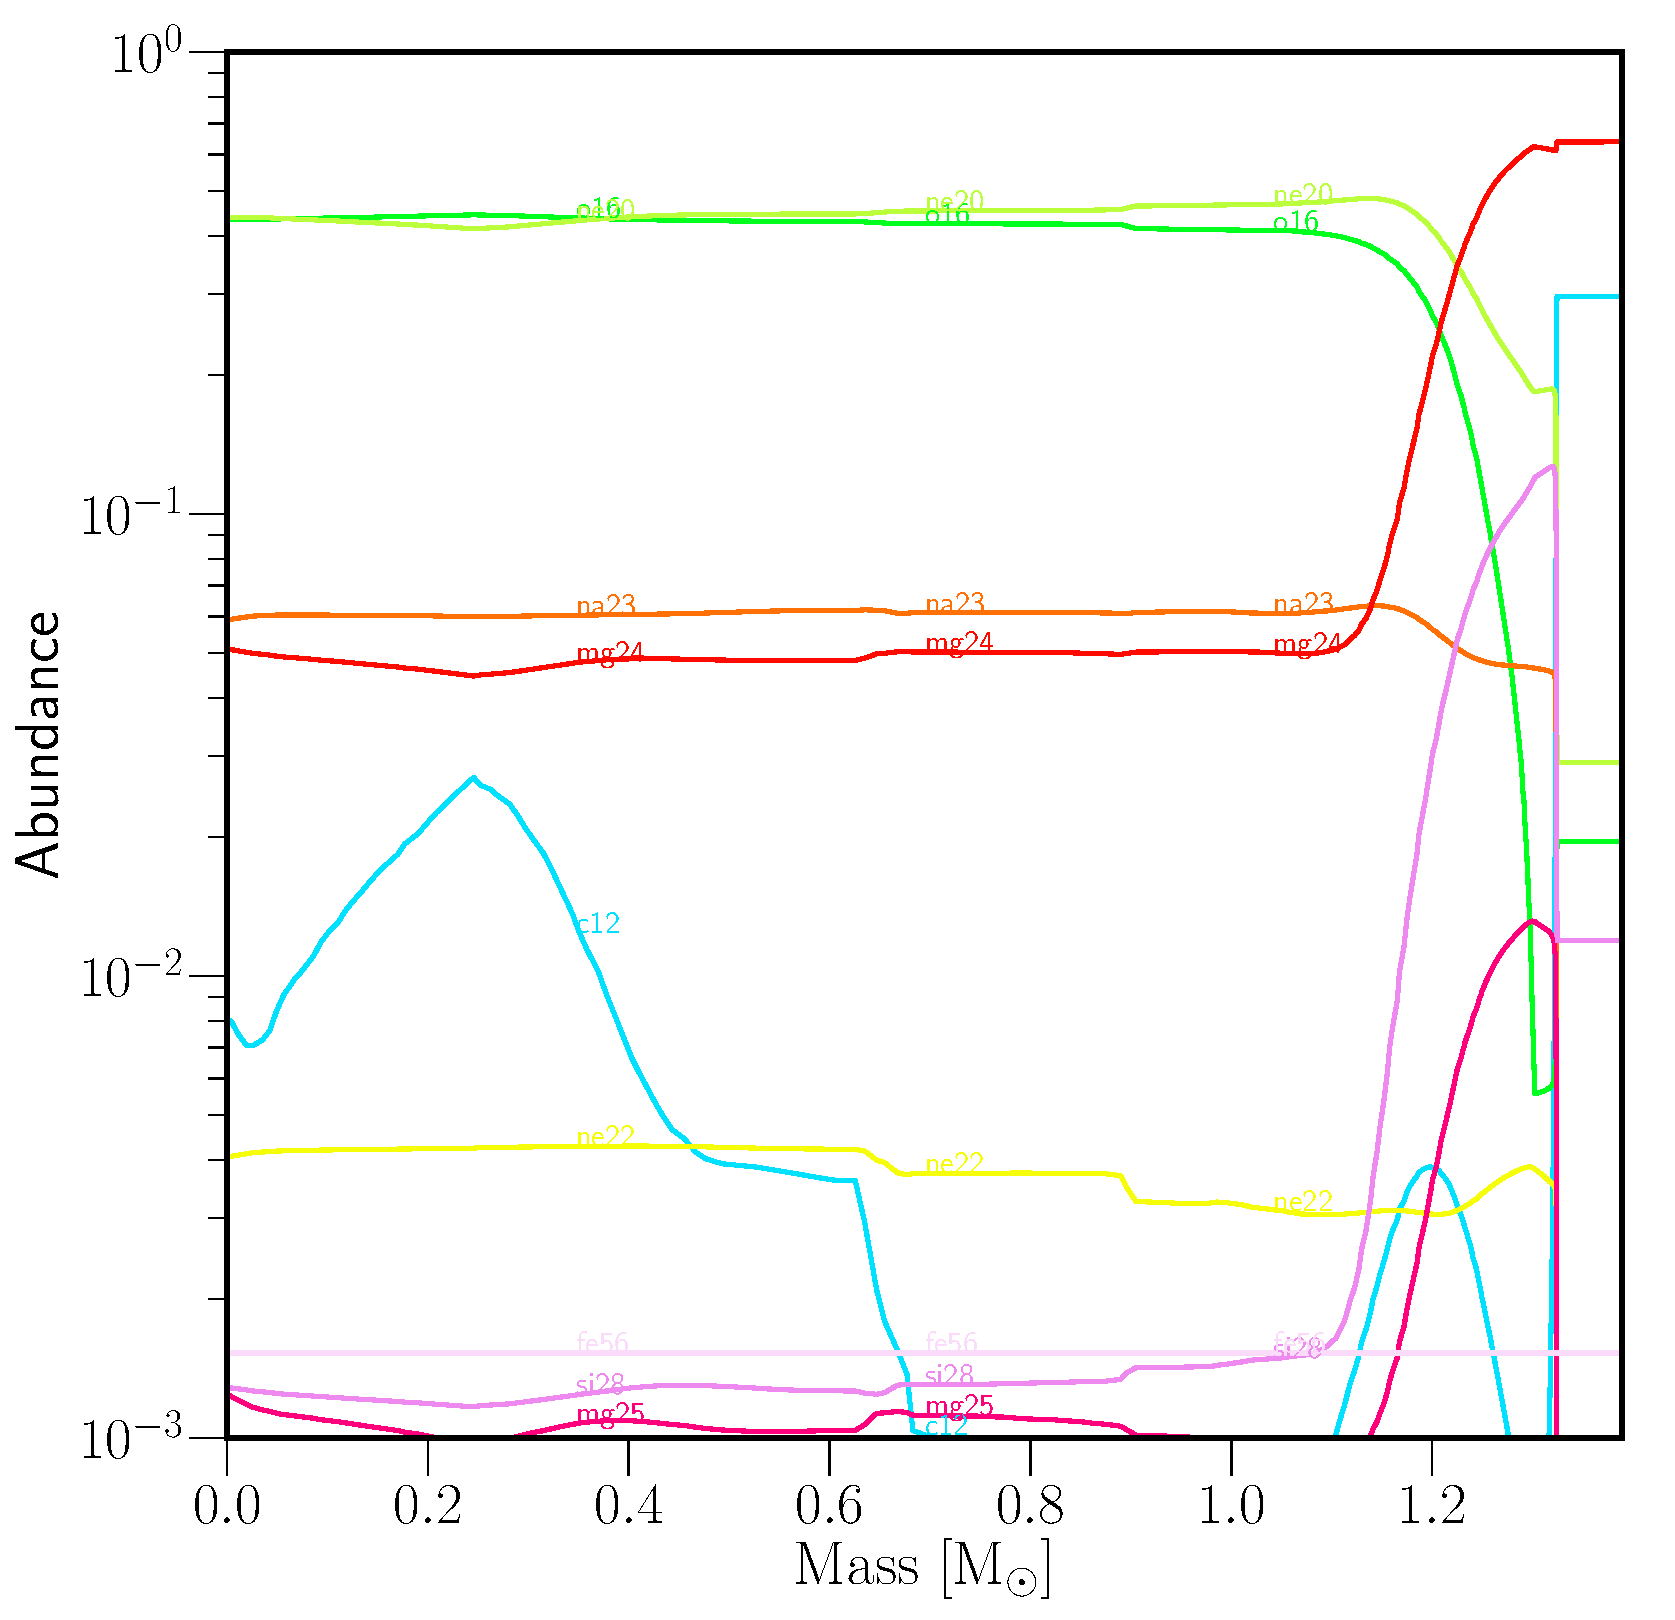
\includegraphics[width=\textwidth]{../figures/chapter4/2p5_logRho_9_abun.pdf}
\caption{Structure of the $2.5 \rm \ M_{\odot},  Z=0.02;f_{OV}=0.0$ stellar model. Residual carbon from previous burning stages is visible.}\label{fig:abun_b}
\end{subfigure}
\hfill
\begin{subfigure}[b]{.45\linewidth}
 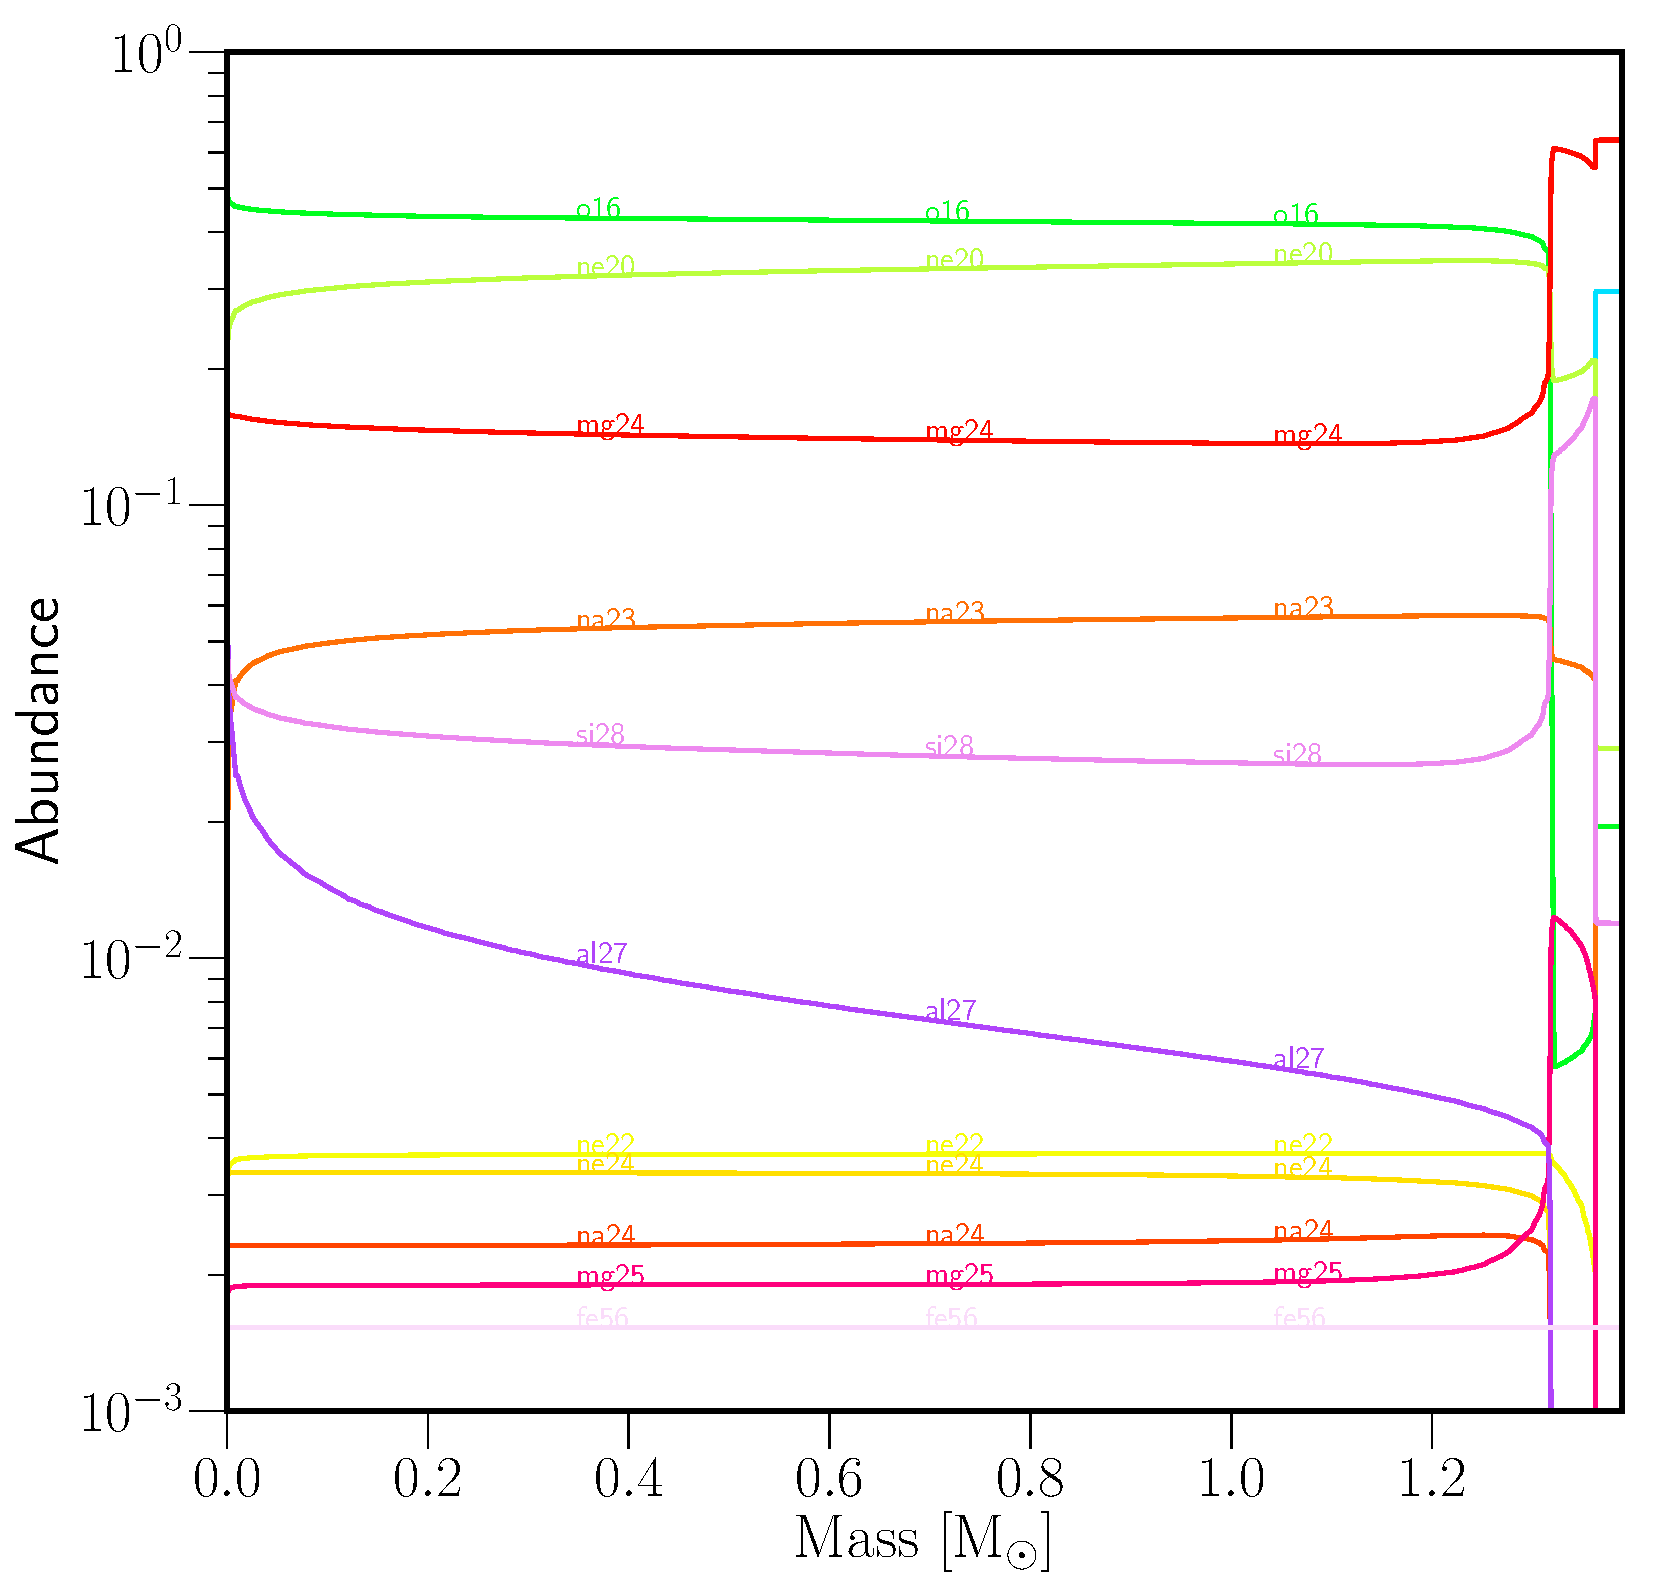
\includegraphics[width=\textwidth]{../figures/chapter4/2p5_final_abun.pdf}
\caption{Final structure of the $2.5 \rm \ M_{\odot}$ stellar model. Residual carbon leads to thermonuclear explosion.}\label{fig:abun_c}
\hfill
\end{subfigure}
\hfill
\begin{subfigure}[b]{.45\linewidth}
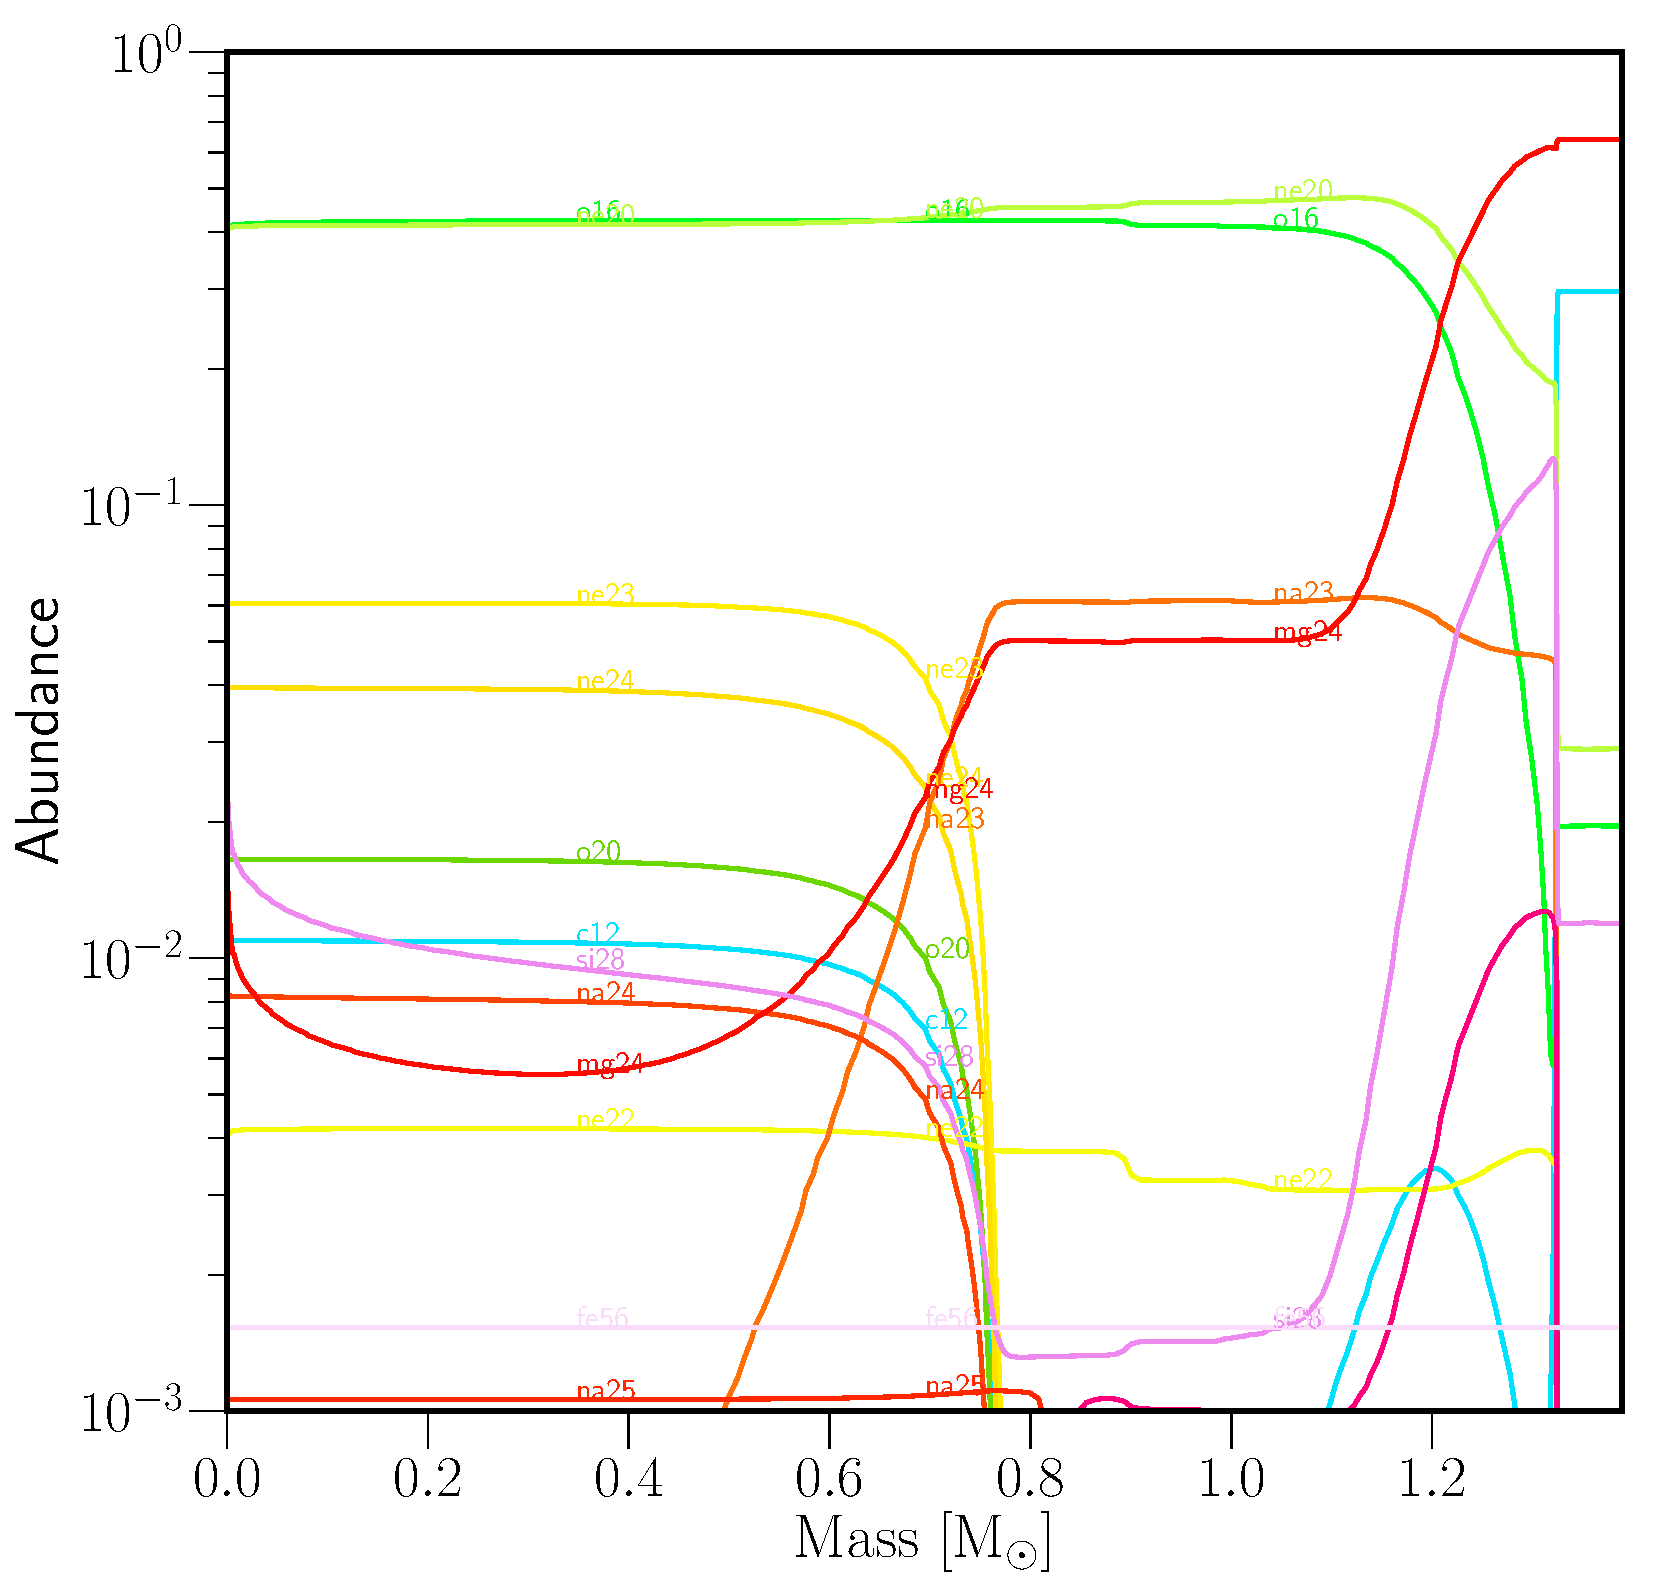
\includegraphics[width=\textwidth]{../figures/chapter4/2p5_abun_carbon_sup.pdf}
\caption{Final structure of the $2.5 \rm \ M_{\odot}$ stellar model, in the case where carbon consuming nuclear reactions have been turned-off.}\label{fig:abun_d}
\end{subfigure}
\hfill
\caption{Abundance profiles of our fiducial models during various evolutionary stages. Panels (a) and (b) refer to the abundace profiles when when $\rm \log(\rho_c / gr \ cm^{-3}) \approx 9.0$ (indicated by the grey circle in Figure \ref{fig:RhoT}). In panel (d), the core reaches the density threshold for e-captures on Ne nuclei to commence, leading to formation of $\rm ^{20}O$, and most likely to an ECSN.}
\label{fig:abundance_profiles}
\end{figure}


\afterpage{%
    \clearpage% Flush earlier floats (otherwise order might not be correct)
    \thispagestyle{empty}% empty page style (?)
    \begin{landscape}% Landscape page
    \label{tab:properties}
        \captionof{table}{Stellar parameters for twenty-two single helium stars, evolved to the pre-SN stage. Models that were able to evolve after oxygen ignition are indicated with an asterisk in the comments. $\rm X_9$ refers to the core mass fraction when $\rm \log(\rho_c/ gr \ cm^{-3}) \approx 9.0$. As ignition density we consider the maximum density before the thermal runaway.} \hspace{5pt}
        \centering % Center table
        \begin{tabular}{ccccccccc}
        \hline \hline \\
        Initial Mass [$\rm M_{\odot}$] & Metallicity ($\rm Z$) & Overshoot ($\rm f_{OV}$) & 
        $\rm X_9(^{12}C)$ & $\rm X_{ig}(^{12}C)$ & $\rm X_{ig}(^{16}O)/X_{ig}(^{20}Ne)$ & 
        $\rm \log(\rho_c^{ig} / gr \ cm^{-3}) = \rho_c^{max}$ & Final core mass [$\rm M_{\odot}$] & Comments \\ \hline \\
            1.8 & 0.02 & 0.014 & 0.254 & 0.25 &  & 9.26 & 1.36 & Hybrid$^{\star}$ \\
1.8 & 0.02 & 0.016 & 0.136 & \nodata & \nodata & \nodata & 1.35 & Hybrid \\
1.9 & 0.001 & 0.016 & 0.014 & \nodata & \nodata & \nodata & 1.35 & ONe core \\
1.9 & 0.02 & 0.014 & 0.061 & \nodata & \nodata &  \nodata & 1.35 & ONe core \\
1.9 & 0.02 & 0.016 & 0.09 & \nodata & \nodata &  \nodata & 1.35 & ONe core \\
2.0 & 0.0001 & 0.016 & 0.0003 & \nodata & \nodata &  \nodata & 1.35 & ONe core \\
2.0 & 0.001 & 0.016 & 0.003 & \nodata & \nodata &  \nodata & 1.35 & ONe core \\
2.0 & 0.02 & 0.016 & 0.05 & \nodata & \nodata &  \nodata & 1.35 & ONe core \\
2.1 & 0.001 & 0.016 & 0.006 & \nodata & \nodata &  \nodata & 1.36 & ONe core \\
2.1 & 0.02 & 0.0 & 0.027 & \nodata & \nodata &  \nodata & 1.37 & ONe core \\
2.1 & 0.02 & 0.016 & 0.01 & \nodata & \nodata &  \nodata & 1.35 & ONe core \\
2.2 & 0.02 & 0.0 & 0.02 & \nodata & \nodata &  \nodata & 1.37 & ONe core \\
2.2 & 0.02 & 0.016 & 0.012 & \nodata & \nodata &  \nodata & 1.35 & ONe core \\
2.3 & 0.02 & 0.0 & 0.011 & 0.01 & 0.85 & 9.75 & 1.37 & ONe core$^{\star}$ \\
2.3 & 0.02 & 0.016 & 0.005 & \nodata & \nodata &  \nodata & 1.37 & ONe core \\
2.4 & 0.001 & 0.0 & 0.006 & \nodata & \nodata &  \nodata & 1.36 & ONe core \\
2.4 & 0.02 & 0.0 & 0.0087 & 0.0066 & 0.87 & 9.75 & 1.37 & ONe core$^{\star}$ \\
2.5 & 0.001 & 0.0 & 0.004 & \nodata & \nodata & \nodata & 1.36 & ONe core \\
2.5 & 0.02 & 0.0 & 0.0062 & 0.0057 & 0.9 & 9.77 & 1.36 & ONe core$^{\star}$ \\
2.6 & 0.001 & 0.0 & 0.0024 & \nodata & \nodata & \nodata & 1.36 & ONe core \\
2.6 & 0.02 & 0.0 & 0.0003 & \nodata & \nodata &  \nodata & 1.36 & ONe core \\
2.7 & 0.02 & 0.0 & 0.0027 & \nodata & \nodata &  \nodata & 1.36 & ONe core \\ \hline
        \end{tabular}
    \end{landscape}
    \clearpage% Flush page
}

% -----------------------------------------------------------
%%              DISCUSSION/FUTURE WORK
% -----------------------------------------------------------
\section{Discussion and Future Work} \label{sec:discussion}

In this work, we demonstrated that the evolution of intermediate mass helium stars (1.8 - 2.7 $\rm M_{\odot}$) can lead to the formation of near-Chandrasekhar mass (C)ONe cores that ignite oxygen at low central densities, triggered by the burning of left-over carbon, resulting in a thermal runaway and avoiding an electron-capture induced collapse. Helium stars in this mass range are a common product of interacting binary systems, and can lose their helium mantle via winds, case-BB Roche lobe overflow, or in a common envelope event, forming a helium-free structure. Lacking an accretion phase from a donor star, our models may contribute significantly to the observed SN\,Ia rate (see Paper I for discussion).

True binary evolution of these cores would help us improve constraints on their progenitor systems, and accurately map mass-loss histories since the binary system may be subjected to early mass transfer episodes leading to effective stripping of the donor star. Moreover, 3D hydrodynamical simulations are required in order to investigate potentially distinct nucleosynthetic yields, and study the energetics of the explosion. Finally, a more extended parameter space that includes parameters that could alter the evolution of our models (e.g. rotation, wind efficiencies) may prove to be essential.





\end{document}